\documentclass{apuntes}

\newcounter{problem}
\newcounter{solution}
\renewcommand{\theenumi}{\alph{enumi}}

\newcommand\Problem[1][]{%
  \color{blue}
  \stepcounter{problem}%
  \ifthenelse{\isempty{#1}}{\textbf{Problema \theproblem.}}{\textbf{Problema #1.}}

  \setcounter{solution}{0}%
}

\newcommand\TheSolution{%
  \color{black}
  \textbf{Solución:}\\%
}

\newcommand\ASolution{%
  \stepcounter{solution}%
  \textbf{Solución \thesolution:}\\%
}


\setlength{\arrayrulewidth}{1mm}
\setlength{\tabcolsep}{18pt}
\renewcommand{\arraystretch}{1.5}


\author{Pedro Valero & Victor de Juan}
\title{Sistemas Informáticos II}
\parindent 0in
\parskip 1em
\makeindex
\begin{document}

\maketitle
\newpage
\tableofcontents

%%%%%%%%%%%%%%%%%%%%%%%%%%%%%%%%%%%%%%%%%%%%%%%%%%%%%%%%%%%%%%%%%%%%%%%%%% PROBLEMA 1

\chapter{Middleware}
Para este tema es importante tener claros varios conceptos que vamos a ir definiendo y explicando poco a poco.

\begin{defn}[Middleware]
Conjunto de aplicaciones encargadas de enlazar los componentes de un sistema distribuido.
\end{defn}

\section{Network Operating System (NOS)}
Este conjunto de aplicaciones está dividido en el protocolo específico del servicio con el que estamos trabajando (ODBC, HTTP, SMTP...), el protocolo de transporte (TCP/IP) y una capa intermedia llamada Network Operating System (NOS).

\begin{defn}[Network Operating System]
Es una extensión del sistema operativo que proporciona transparencia al cliente, para que éste realice las llamadas como si fueran locales.
\end{defn}

Algunas de las maneras de proporcionar transparencia del NOS según \concept{RM-ODP} (Open Distributed Processing Reference Model) son
\begin{itemize}
\item Ubicación: Ocultar dónde reside cada recurso (y permite que éste se mueva, incluso mientras está siendo utilizado).
\item Persistencia: Ocultar tanto la activación y desactivación de objetos como sus fallos y recuperaciones mediante la replicación.
\item Concurrencia: Ocultar la utilización de recursos concurrentes.
\item Prestaciones: Escalar el tamaño y reconfigurar el sistema para mejorar sus prestaciones según varía la carga de trabajo.
\item Espacio de nombres:
\item SSO: Single Sign On - Un único usuario y contraseña para todo el sistema.
\item Tiempo: Todos los componentes deben estar sincronizados.
\item Protocolos: Idéntica interfaz de programación para todos los protocolos de transporte.
\end{itemize}

Debido a que la representación interna de los datos es dependiente del ordenador (hardware o sistema operativo) es necesario definir un mecanismo para que, independientemente de la plataforma, la comunicación sea posible. Algunos métodos son utilizar estándares de \textbf{codificación de caracteres} (ISO-8859-1,UTF-8), \textbf{XML}, sistemas propios de aplicaciones (\textbf{RPC,XDR}) o un estándar \textbf{Abstract Synyax Notation} (con una gramática y reglas para codificar los datos).


\section{Servicios de transporte}

Una vez hablado del NOS, vamos a ver unos conceptos de  servicios de transporte del middleware.

Lo primero es recordar que hay 2 modelos de interacción, \textbf{síncrono} o \textbf{asíncrono}. Además de estos modelos, las interacciones pueden ser de tres tipos.
\begin{itemize}
	\item \textbf{R:} Petición. (El cliente hace una petición sin esperar respuesta, por ejemplo para cerrar la conexión)
	\item \textbf{RR:} Petición → Respuesta.
	\item \textbf{RRA:} Petición → Respuesta → ACK.
\end{itemize}

\subsection{API directa}

\begin{defn}[APIs directas]
API viene de \textit{Application Programming Interface} (Interfaz de programación de aplicaciones).

La utilización de APIs directas es la utilización de una interfaz de programación para acceder a unos servicios (proporcionados por la aplicación).
\end{defn}

Habitualmente son servicios de nivel de transporte o sesión. La ubicación de extremos no es transparente para el programa, ya que necesitas saber dónde está la interfaz para poder utilizarla. Para ver un ejemplo de API, consultar: \href{https://apigee.com/OneDrive/embed/console/OneDrive}{API de OneDrive}.

\subsection{Sockets}

Son la leche porque proporcionan mucha transparencia: podemos comunicarnos entre procesos sin tener ni idea de nada, simplemente es como escribir en un fichero (de hecho, si recordamos de Redes II un socket es directamente un descriptor de fichero en Linux).

Aunque ya deberíamos saberlo, incluimos un par de esquemas (sacados de las transparencias) en los que vemos cómo establecer una comunicación orientada a conexión (\ref{SocketConexion}) y una comunicación no orientada a conexión (\ref{SocketNoConexion})


\begin{figure}[hbtp]
\centering
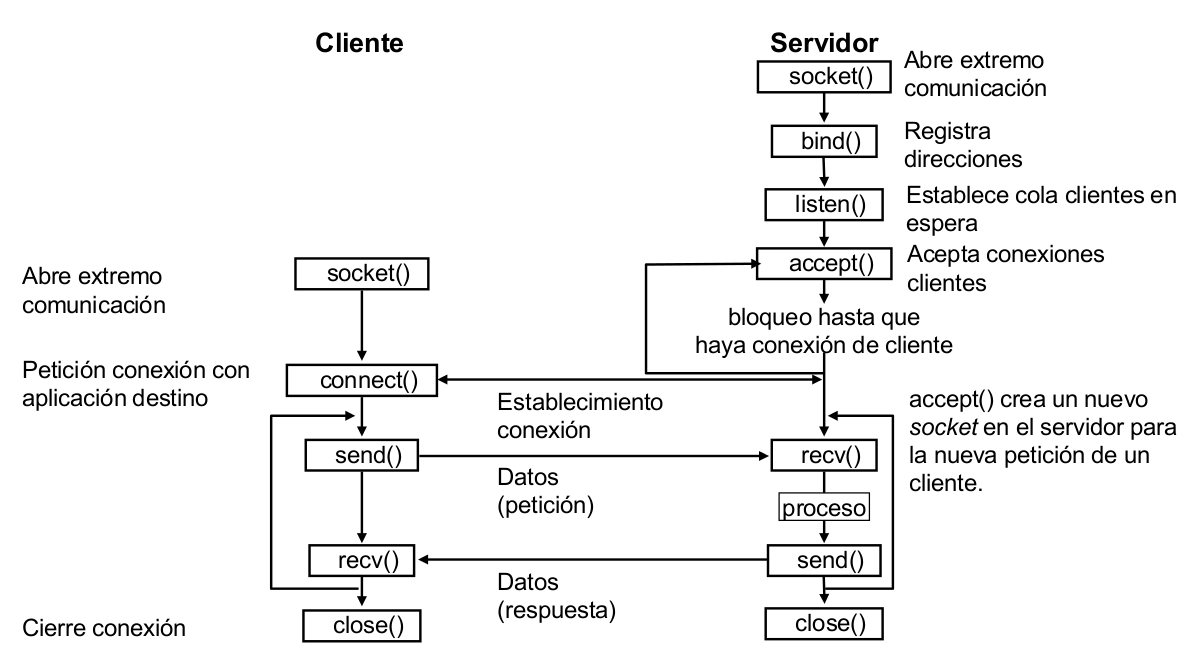
\includegraphics[width=1\textwidth]{img/SocketConexion.png}
\caption{Comunicación orientada a conexión.}
\label{SocketConexion}
\end{figure}

\begin{figure}[hbtp]
\centering
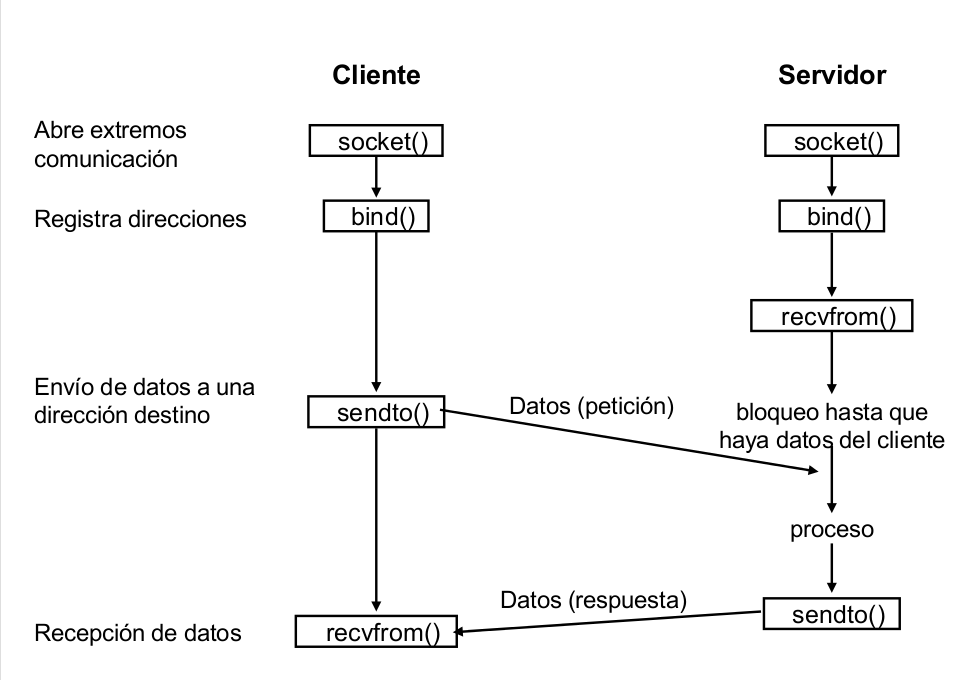
\includegraphics[width=1\textwidth]{img/SocketNoConexion.png}
\caption{Comunicación No Orientada a conexión.}
\label{SocketNoConexion}
\end{figure}
\newpage
\section{Modelos de servicios distribuidos}

La base de este curso es cómo dar servicio a muchos clientes. Si tenemos una web a la que se conectan 10 personas, nos vale con cualquier ordenador, pero ¿Cuánta gente usa google? Ni de coña google tiene un único servidor haciendo todo, tiene que tener los \textbf{servicios distribuidos}. A lo largo de esta sección iremos viendo muchas de las maneras de llevar esto a cabo.

\subsection{RPC - Remote Procedure Calls}
Este modelo se basa en realizar llamadas a funciones como si fueran locales, así el procesamiento de esa función no se realiza en local sino en remoto y nos ahorramos recursos de procesamiento.

Para el funcionamiento de RPCs necesitamos unos componentes intermedios llamados \concept{Stub}. En el siguiente diagrama se entiende perfectamente el funcionamiento de los RPCs.
\begin{figure}[htb]
\centering
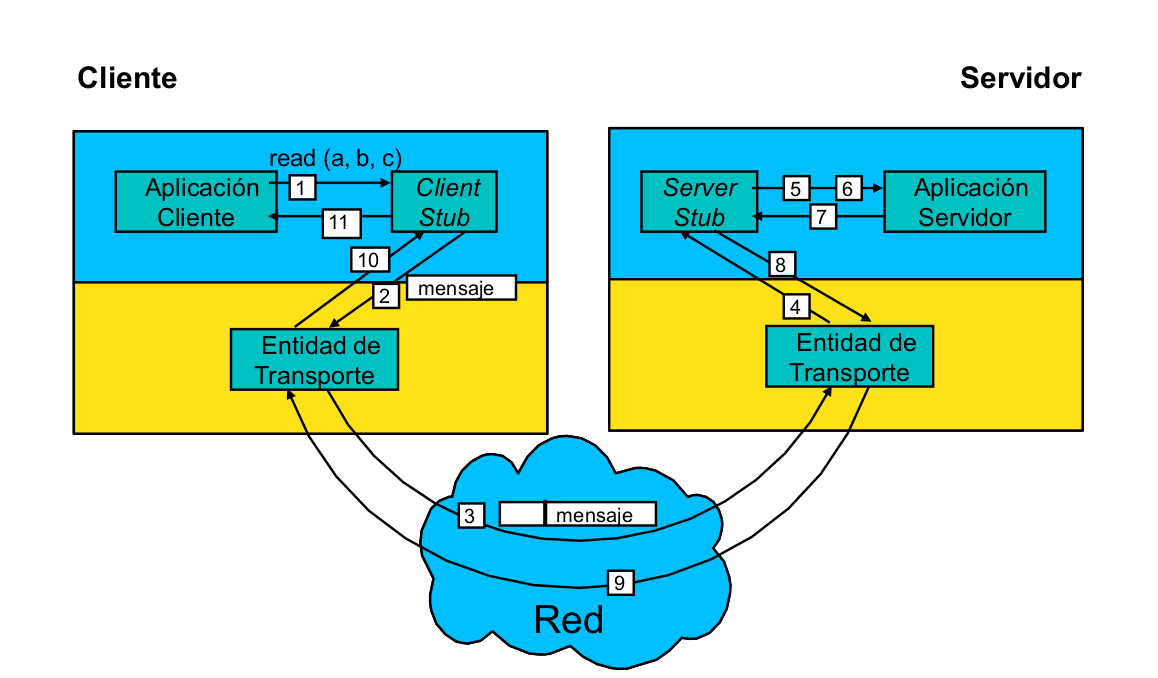
\includegraphics[width=0.9\textwidth]{img/RPC.png}
\caption{Funcionamiento de una llamada RPC.}
\label{RPCimg}
\end{figure}
\newpage

\obs La espera del cliente es \textbf{bloqueante}.

\obs Una ventaja realmente interesante de esto es la transparencia de representación de los datos. RPC (y los stubs intermedios) permiten que un cliente que utiliza Big Endian pueda pasarle los parámetros a una función que se ejecute en un servidor que utiliza Little Endian. Esta \textit{transformación} de los datos de un sistema de codificación al otro se llama \concept{Marshalling} (el codificarlos para enviar) y \concept{Unmarhsalling} (descodificarlos al recibirlos). Ambos stubs tienen que hacer marshalling y unmarshalling al enviar y recibir mensajes respectivamente.

\paragraph{Problemas de RPC}
\begin{itemize}
	\item No existe el paso de parámetros por referencia.
	\item Hay que conocer de antemano dónde está el servidor exáctamente y en qué puerto escucha.
	\subitem Para saber el puerto en el que el servidor está escuchando, éste tiene que registrarse en un \concept{PortMapper} al que el cliente pregunta por el puerto.
 	\item Tras un \textit{Time Out} No se sabe si la llamada se ha ejecutado o no. Para intentar mitigar este problema en algunos casos, encontramos estrategias distintas en las llamadas RPC:
		\subitem Ejecución Exactamente una vez.
		\subitem Ejecución Como máximo una vez.
		\subitem Ejecución Al menos una vez.\\
	Para solventar esto es necesario también saber si las operaciones son \concept{operaciones de RPC idempotentes} (se pueden ejecutar cualquier número de veces) o no\footnote{Por ejemplo un cálculo $4+4$ lo puedes ejecutar todas las veces que quieras, pero un insert en una base de datos no}.
	\item Es necesaria una representación de datos compartida por los stubs.
	\item Seguridad. ¿Y si el servidor ha sido comprometido y me va a devolver datos que me hagan mal?
\end{itemize}


\paragraph{SUN RPC: } Una de las implementaciones más comunes de RPC es \concept{Sun RPC}. Vamos a estudiarla un poco más en detalle.


Tiene 3 componentes:
\begin{itemize}
	\item \concept{XDR} Lenguaje de definición de tipos de datos. Tiene una sintaxis similar a C, pero es sólo de definición de datos, no de programación
	\item \textbf{Especificación de RPC: } Genera los \textit{stubs} y el fichero de interfaz (para ser incluido al programar)
	\item \textbf{Librería de implementación}
\end{itemize}

Sólo por si interesa, incluimos un esquema de cómo funciona y qué ficheros se generan en la codificación de un servicio utilizando RPC.


\begin{figure}[htb]
\centering
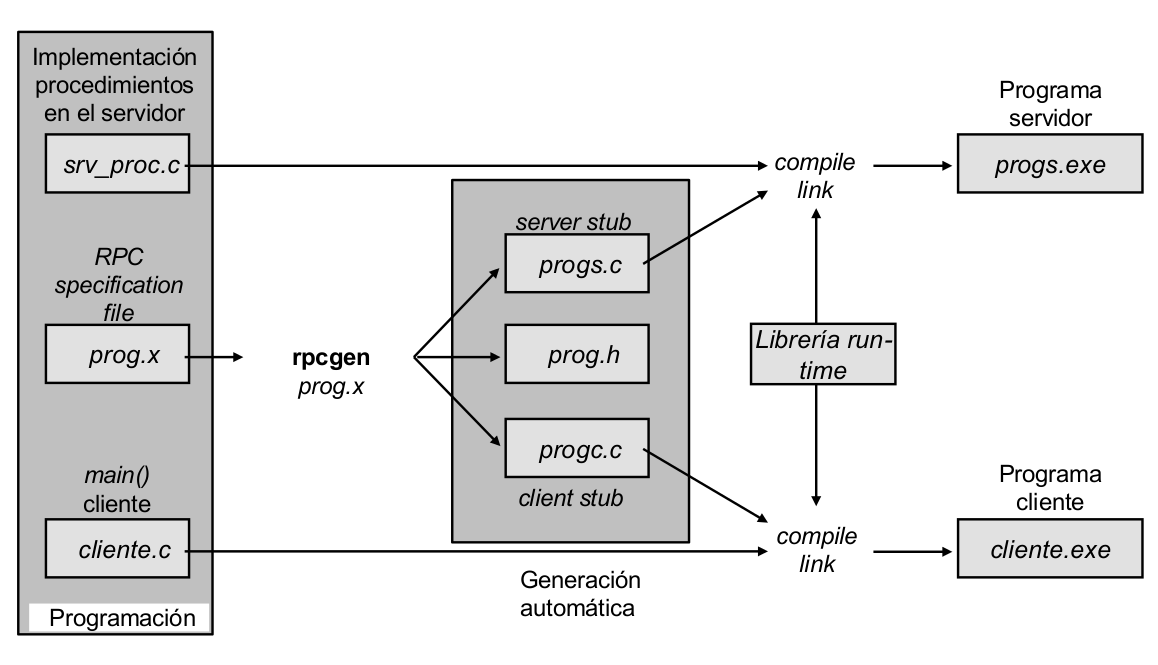
\includegraphics[width=1\textwidth]{img/SUNRPC.png}
\caption{Compilación y generación de código para Sun RPC.}
\label{SunRPC}
\end{figure}

\paragraph{Algunas diferencias entre RPCs}
\begin{itemize}
	\item Parámetros: Aunque en general soporten múltiples parámetros (\concept{Apollo RPC} por ejemplo), Sun RPC sólo tiene un único parámetro, tanto de entrada como de salida (obviamente pueden ser estructuras).
	\item Marshalling: En general lo hace el RPC, aunque en Sun RPC el marshalling que se realiza es mínimo. Es responsabilidad del usuario tener cuidado con eso.
\end{itemize}

Comentamos que Apollo RFC tiene su propio lenguaje de representación de datos, \textit{Network Data Representation} \concept{NDR} (como el XDR de Sun RPC). Apollo tiene también un lenguaje de representación de interfaces \concept{NIDL} (\textit{Network Interface Definition Language}).

\subsection{Web Services (SOAP-WSDL-UDDI)}
Es un modelo de uso de la Web. La idea es tener servidores que ofrecen servicios (localizar geográficamente a través de la IP, ofrecer información de finanzas...) y que cualquiera puede requerir esos servicios. ¿Qué diferencia tiene con RPC? Que en RPC el programador tiene que codificar el lado del servidor y tener conciencia de como funciona, mientras que con los WebServices, el programador que está haciendo un cliente puede utilizar los servicios que le proporciona un servidor que otro programador haya hecho en cualquier otro momento.

Añade un nivel más de transparencia, ya que el programador del cliente no tiene ni idea de cómo funciona el WebService.

La \textbf{función del middleware} aquí es proporcionar funcionalidad para publicar los servicios que ofreces y descubrir los nuevos servicios que vayan surgiendo. Además, tiene que permitir que los servidores soliciten servicios también (multi-\textit{tier}).

\paragraph{Complementos de los Web Services} \concept{OASIS} (Organization for the Advancement of Structured Information Standards) está trabajando (y ha trabajado) en estandarizar una serie de complementos útiles para la mejor utilización de los Web Services y una serie de familia de especificaciones:
\begin{itemize}
\item Complementos:
	\subitem Seguridad.
	\subitem Fiabilidad.
	\subitem Addresing: describir las direcciones de emisor y receptor de un mensaje dentro del propio mensaje.
	\subitem Transaction.
\item \concept{WSRL} - Web Services Resource Framework.
	\subitem WS-Resource (Conjunto de un recurso y un Web Service a través del cual se accede a él.
	\subitem WS-ResourceProperties
	\subitem WS-ResourceLifetime
	\subitem WS-BaseFaults (mecanismo extensible para gestionar errores)
	\subitem WS-ServiceGroup
\end{itemize}

Los WebServices necesitan de 3 protocolos estándares. En el siguiente gráfico se muestran los componentes y protocolos de comunicación utilizados en los WebServices.


\begin{figure}[htb]
\centering
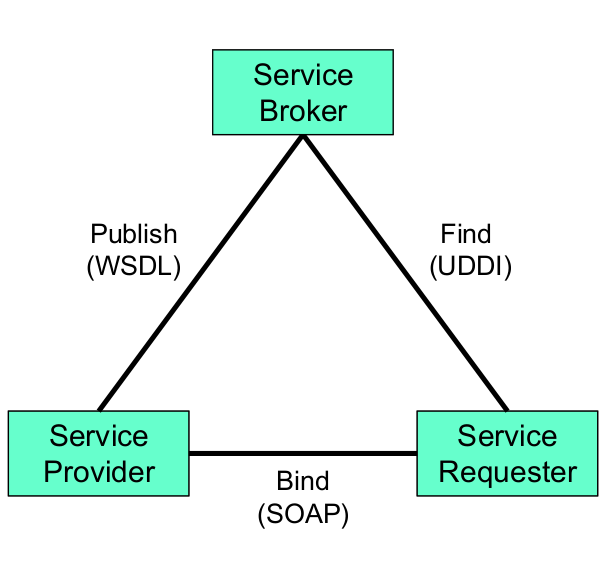
\includegraphics[width=0.9\textwidth]{img/WS.png}
\caption{Componentes de un WS para su funcionamiento.}
\label{WSimg}
\end{figure}


\subsubsection{SOAP}
\begin{defn}[SOAP]
(siglas de Simple Object Access Protocol) Es un protocolo estándar que define cómo dos objetos en diferentes procesos pueden comunicarse por medio de intercambio de datos XML.

Es independiente de la plataforma y el lenguaje de programación y, aunque se puede usar en distintos sistemas de mensajes y sobre distintos protocolos de transporte, su uso principal es transportar RPCs sobre HTTP.
\end{defn}

Un mensaje SOAP es un documento XML ordinario con una estructura definida en la especificación del protocolo. Dicha estructura la conforman las siguientes partes:
\begin{itemize}
\item \textbf{Envelope (obligatoria)}: Raíz que da la estructura, es la parte que identifica al mensaje SOAP como tal.
\item \textbf{Header}: Esta parte es un mecanismo de extensión ya que permite enviar información relativa a cómo debe ser procesado el mensaje. Es una herramienta para que los mensajes puedan ser enviados de la forma más conveniente para las aplicaciones. El elemento "Header" se compone a su vez de "Header Blocks" que delimitan las unidades de información necesarias para el header.
\item \textbf{Body (obligatoria)}: Contiene la información relativa a la llamada y la respuesta.
\item \textbf{Fault}: Bloque que contiene información relativa a errores que se hayan producido durante el procesado del mensaje y el envio desde el "SOAP Sender" hasta el "Ultimate SOAP Receiver"
\end{itemize}

\subsubsection{WSDL}
\begin{defn}[WSDL]
WSDL son las siglas de Web Services Description Language, un formato XML que se utiliza para describir servicios Web.

WSDL describe la interfaz pública de los servicios Web. Está basado en XML y describe la forma de comunicación, es decir, los requisitos del protocolo y los formatos de los mensajes necesarios para interactuar con los servicios listados en su catálogo. Las operaciones y mensajes que soporta se describen en abstracto y se ligan después al protocolo concreto de red y al formato del mensaje
\end{defn}

Estructura de una declaración WSDL
\begin{itemize}
\item \textbf{definitions}: Elemento raíz que contiene el resto. Define su
nombre y los espacios de nombres que utiliza.
\item \textbf{types}: Tipos de datos utilizados entre cliente y servidor. Usa
W3C XML Schema (XSD) por defecto.
\item \textbf{message}: Declaraciones de mensajes empleados para
peticiones y respuestas y los elementos que los forman.
\item \textbf{portType}: Operaciones soportadas y encadenamiento de
mensajes que implica su ejecución.
\item \textbf{binding}: Modo en que los mensajes se transmiten sobre un
protocolo de RPC, con extensiones específicas para SOAP.
\item \textbf{service}: Contiene la información de la dirección en la que se
localiza el servicio.

\end{itemize}

\subsubsection{UDDI}
\begin{defn}[UDDI]
UDDI son las siglas del catálogo de negocios de Internet denominado Universal Description, Discovery and Integration. El registro en el catálogo se hace en XML. UDDI es una iniciativa industrial abierta (sufragada por la OASIS) entroncada en el contexto de los servicios Web.
\end{defn}

Consta de 3 partes: \textbf{modelo de datos} (esquema XML), la \textbf{API} (RPCs con SOAP para registrar y buscar servicios) y los \textbf{Cloud Services} (los servidores que proporcionan el servicio).

El registro de un negocio en UDDI distingue tres categorías de datos:
\begin{itemize}
\item \textbf{Páginas blancas}. Dirección, contacto y otros identificadores conocidos.
\item \textbf{Páginas amarillas}. Categorización industrial basada en taxonomías.
\item \textbf{Páginas verdes}. Información técnica sobre los servicios que aportan las propias empresas.
\end{itemize}
UDDI es uno de los estándares básicos de los servicios Web cuyo objetivo es ser accedido por los mensajes SOAP y dar paso a documentos WSDL, en los que se describen los requisitos del protocolo y los formatos del mensaje solicitado para interactuar con los servicios Web del catálogo de registros.


\paragraph{Ventajas e inconvenientes de los Web Services}

\textbf{Ventajas}
\begin{itemize}
\item Aportan interoperabilidad entre aplicaciones de software independientemente de sus propiedades o de las plataformas sobre las que se instalen.
\item Los servicios Web fomentan los estándares y protocolos basados en texto, que hacen más fácil acceder a su contenido y entender su funcionamiento.
\item Permiten que servicios y software de diferentes compañías ubicadas en diferentes lugares geográficos puedan ser combinados fácilmente para proveer servicios integrados.
\end{itemize}


\textbf{Inconvenientes}
\begin{itemize}
\item Para realizar transacciones no pueden compararse en su grado de desarrollo con los estándares abiertos de computación distribuida como CORBA (Common Object Request Broker Architecture).
\item Su rendimiento es bajo si se compara con otros modelos de computación distribuida, tales como RMI (Remote Method Invocation), CORBA o DCOM (Distributed Component Object Model). Es uno de los inconvenientes derivados de adoptar un formato basado en texto. Y es que entre los objetivos de XML no se encuentra la concisión ni la eficacia de procesamiento.
\item Al apoyarse en HTTP, pueden esquivar medidas de seguridad basadas en firewall cuyas reglas tratan de bloquear o auditar la comunicación entre programas a ambos lados de la barrera.
\end{itemize}

\subsection{REST}
\begin{defn}[REST]
Si bien el término REST se refería originalmente a un conjunto de principios de arquitectura, en la actualidad se usa en el sentido más amplio para describir cualquier interfaz web simple que utiliza XML y HTTP, sin las abstracciones adicionales de los protocolos basados en patrones de intercambio de mensajes como el protocolo de servicios web SOAP.

Es posible diseñar sistemas de servicios web de acuerdo con el estilo arquitectural REST de Fielding y también es posible diseñar interfaces XMLHTTP de acuerdo con el estilo de llamada a procedimiento remoto (RPC), pero sin usar SOAP.

Estos dos usos diferentes del término REST causan cierta confusión en las discusiones técnicas, aunque RPC no es un ejemplo de REST.
\end{defn}

Al trabajar con REST se considera que el sistema se compone de \textbf{recursos}, es decir, elementos que deben ser accedidos en el sistema distribuído y a los que se accede a través de su identificador global \concept{URI}.

La idea es utilizar los métodos de HTTP para acceder a los recursos y servicios del servidor. El servidor define su interfaz normalmente utilizando \concept{WADL} \textit{Web Application Description Language}. El programador del cliente tiene que saberse la especificación concreta, y saber qué objetos recibe qué peticiones.

Para entender mejor REST, miramos el ejemplo de la API de onedrive:

\begin{figure}[hbtp]
\centering
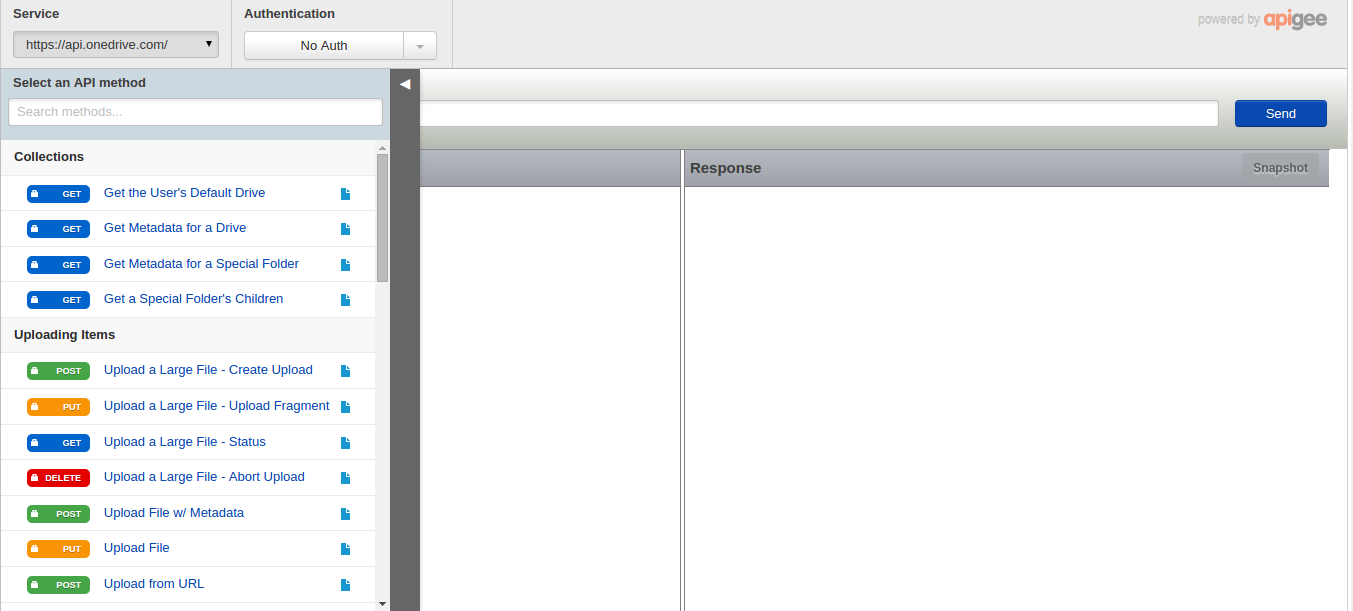
\includegraphics[width=1\textwidth]{img/REST.png}
\caption{API de OneDrive utilizando REST.}
\label{REST}
\end{figure}

Aquí están descritas las posibilidades que existen en el servidor de OneDrive. Con simples peticiones HTTP podemos funcionar. La petición \textit{https://api.onedrive.com/v1.0/drive/} (un GET de HTTP normal) nos devolvería el directorio con las carpetas que tiene el usuario con el que nos hayamos autenticado antes. ¿Cómo autenticarse? Con una petición POST con los datos pertinentes. ¿Y cómo nos devuelve los datos? Lo más habitual es en formato \textbf{JSON} aunque también puede ser en XML.

La utilización de HTTP y JSON/XML hace posible la programación de clientes en cualquier plataforma y es una comunicación más ligera que SOAP. Un inconveniente es que es menos ``transparente''\footnote{transparente en el sentido de que no te enteras de nada. Para utilizar REST tienes que saber más del servicio que utilizas.}.

\textbf{REST es una arquitectura, no un estándar.}


\subsection{Comuncación mediante colas de mensajes}

\begin{defn}[MOM]
Message Oriented Middleware.

Es un proceso asíncrono en el que se genera un mensaje, se encola y se sigue lo que se estaba. Como mandar un correo electrónico, que se encola en la bandeja de entrada y tu sigues trabajando.
\end{defn}

Las conexiones en colas de mensajes pueden ser 1-1, 1-N, N-1 y N-M.

\paragraph{Situaciones ideales}
\begin{itemize}
 	\item Conexiones no permanentes y costosas.
 	\item Múltiples servidores procesando mensajes de clientes.
 	\item Llegada de mensajes impredecibles o en ráfagas
 	\item Sistemas de tipo publicación/suscripción.
 \end{itemize}
 \obs Permite balanceo automático de carga en un sistema distribuido. Se pueden procesar los mensajes con prioridades, no necesariamente FIFO.

Vamos a ver algunos ejemplos de gestores de colas.
\subsubsection{IBM Web Sphere MQ}
Es el MOM más extendido. Es multiplataforma y multiprotocolo.


\concept{IBM Sphere MQ} está formado por
\begin{itemize}
	\item Gestores de colas, encargados de manejar el envío y recepción de los mensajes, además de crear y gestionar el resto de los elementos.

	Tiene una API con
	\subitem Message Queuing Interface (MQI)
	\subitem Application Messagin Interface (AMI)
	\subitem Java Messaging Services (JMS)
	\item Colas de mensajes de múltiples tipos.
	\item Canales de comunicación: Conexiones unidireccionales entre gestores de colas.
\end{itemize}

A continuación mostramos un esquema de funcionamiento de un sistema de mensajería de colas:


\begin{figure}[hbtp]
\centering
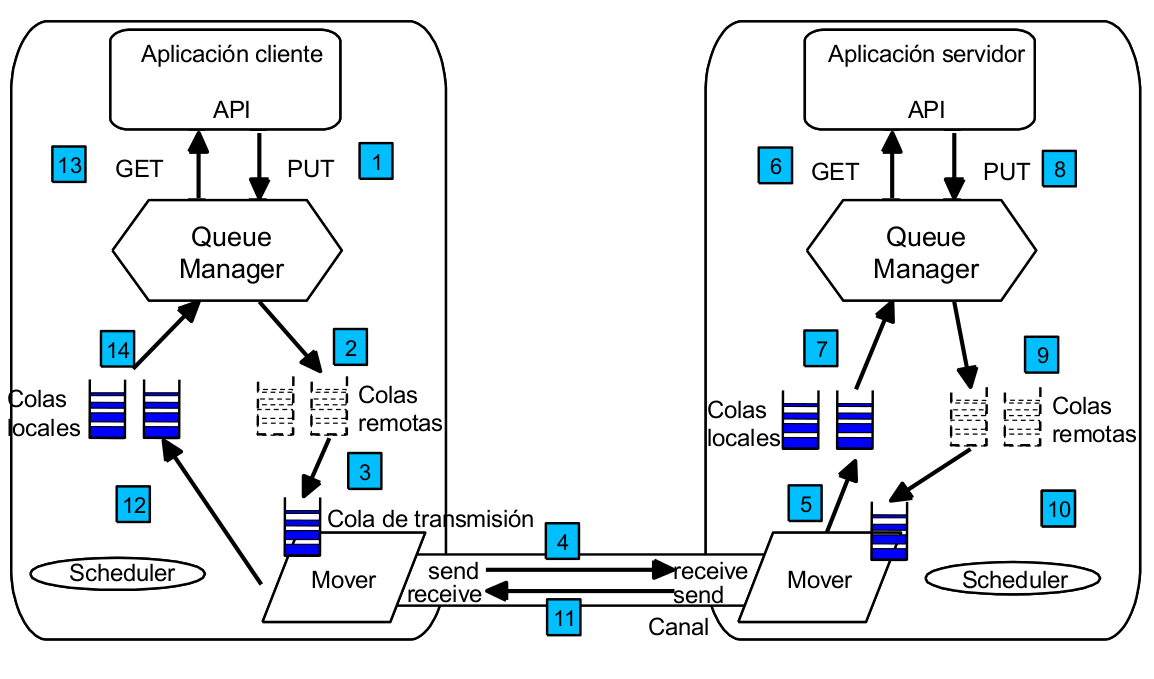
\includegraphics[width=1\textwidth]{img/MOMGen.png}
\caption{Sistema de mensajería de colas.}
\label{MOMGen}
\end{figure}
\newpage

Vemos que se distinguen 3 tipos de colas, las locales (del propio sistema) y las remotas, que el sistema reconoce que pertenecen a otro sistema y entonces el mensaje tiene que ser enviado al sistema al que pertenece la cola remota.

Además de estos 3 tipos de colas (locales, remotas y de transmisión) podemos definir en nuestras colas un par de propiedades: persistentes o temporales (en el almacenamiento de los mensajes) y estáticas (definidas permanentemente) o dinámicas (creadas por aplicaciones). Las colas dinámicas se crean a partir de una cola modelo.

También existen las colas de activación, y de cartas muertas (con mensajes que no se han podido entregar)


En resumen, los tipos de colas pueden ser:
\begin{itemize}
	\item Local - remota.
	\item Persistente - temporal.
	\item Estática - dinámica.
	\item Activación.
	\item Cartas muertas.
	\item Transmisión.
\end{itemize}

\begin{example}
Una de las utilidades de MOM son los servicios de publicación/suscripción. A continuación incluimos un esquema que muestra perfectamente cómo funcionan este tipo de sistemas.


\begin{figure}[hbtp]
\centering
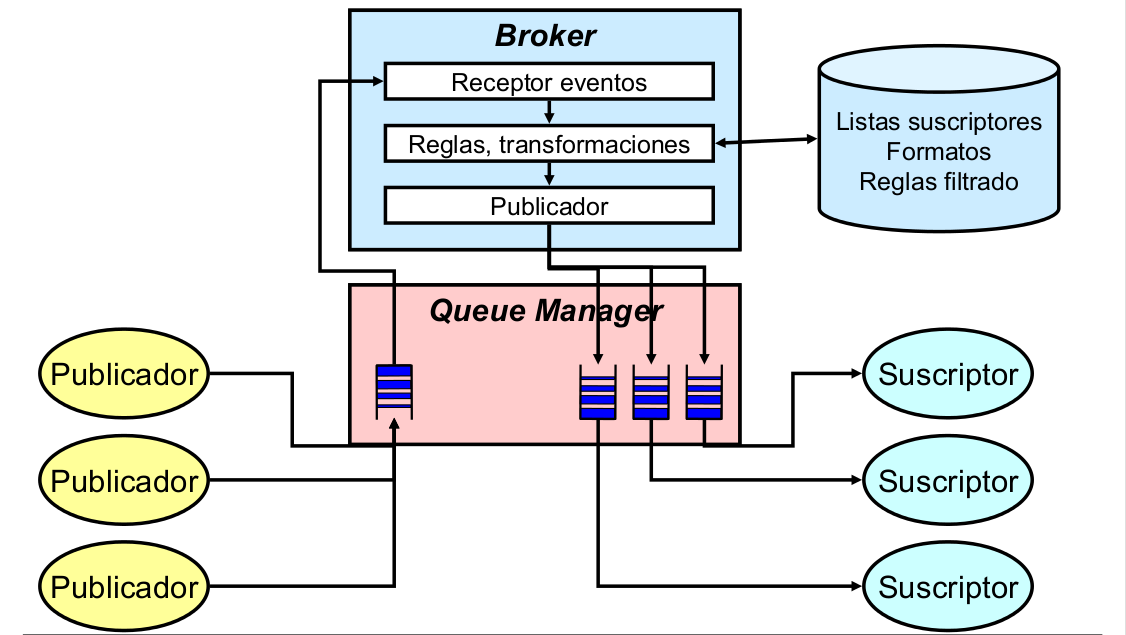
\includegraphics[width=1\textwidth]{img/PubSusc.png}
\caption{Sistema publicador/suscriptor.}
\label{PubSusc}
\end{figure}
\newpage
\end{example}


\section{Services Oriented Architecture SOA}
\subsection{ESB - Enterprise Services Bus}

Extendiendo el modelo de publicador/suscriptor tenemos un ESB. El ESB actúa como proceso centralizador de solicitudes de los clientes (normalmente mensajes o solicitudes de ejecución de acciones tipo RPC – Web Services) para su distribución a los servidores.


\begin{figure}[hbtp]
\centering
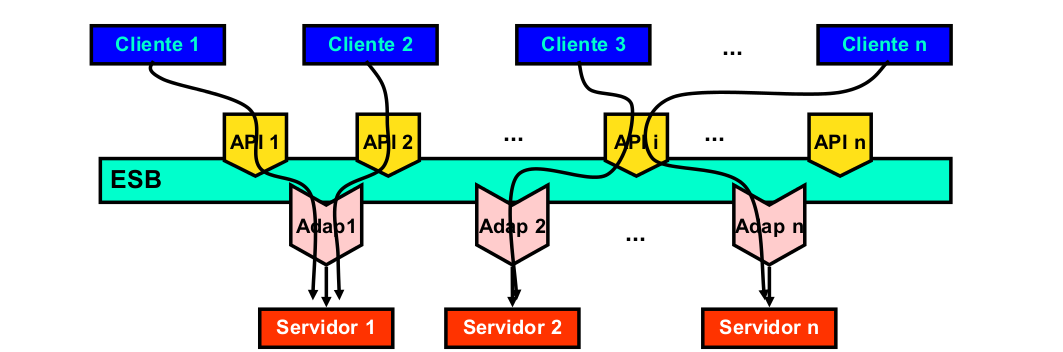
\includegraphics[width=1\textwidth]{img/ESB.png}
\caption{Enterprise Service Bus.}
\label{ESB}
\end{figure}

A continuación, estudiamos las ventajas e inconvenientes que puede tener un sistema como este:
\paragraph{Ventajas:}
\begin{itemize}
\item Adaptación rápida en entornos existentes.
\item Flexibilidad. Fácil de adaptar a nuevos requerimientos.
\item Basado en estándares.
\item Existencia de tipos de servicios y APIs predefinidas y listas para su uso.
\item Convierte tareas de programación en configuración (manipulación de datos, por ejemplo).
\item Facilita la gestionabilidad del sistema, al proporcionar un punto único de control para todos los intercambios.
\end{itemize}
\paragraph{ Inconvenientes:}
\begin{itemize}
\item Posible punto único de fallo.
\item Fácil saturación del ESB a cargas altas de comunicación.
\item Sin una planificación correcta de APIs y conectores no evita la conexión lógica punto a punto entre clientes y servidores, sólo la física.
\item Requiere más sistemas en ejecución, para soportar el propio ESB.
\item Introducción de un elemento adicional en la cadena de procesamiento, con lo cual el rendimiento se puede ver afectado.
\item Escasas ventajas para entornos sencillos. Estas se ven más en situaciones complejas, con muchos tipos de clientes y servidores.
\end{itemize}

\subsection{RMI - Remote Method Invocation}

Igual que en programación estructurada podíamos ejecutar funciones remotamente (con RPC), con la programación orientada a objetos (POO) también podemos tener localmente una referencia a un objeto remoto y ejecutar métodos del objeto remoto. Para ello es necesario disponer de un middleware espefícico, con unos módulos de comunicación y de referencia remota.


\begin{figure}[hbtp]
\centering
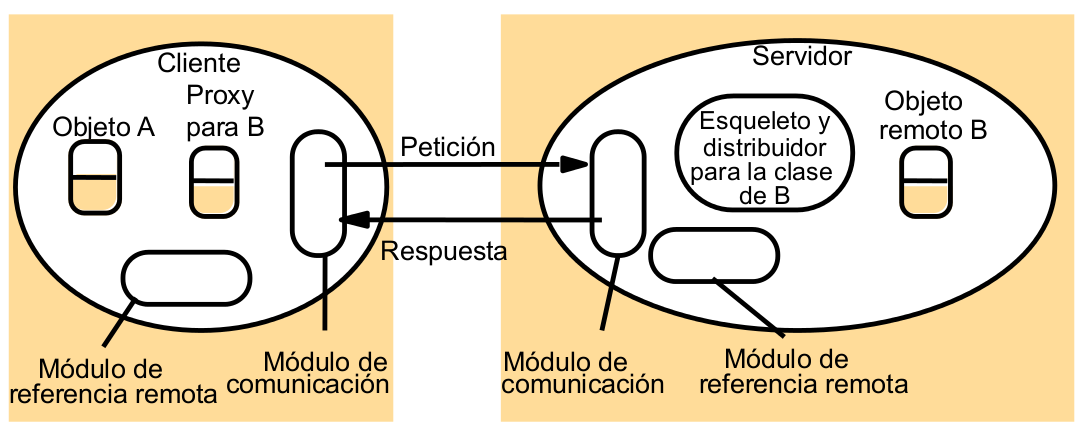
\includegraphics[width=1\textwidth]{img/RMI.png}
\caption{Esquema de funcionamiento de RMI.}
\label{RMI}
\end{figure}

En RMI también es necesario realizar marshalling y unmarshalling. El componente encargado de hacerlo es el esqueleto (del objeto remoto).

El otro componente que merece mención es el módulo de la referencia remota. El objeto que tiene el cliente es una referencia que el módulo de referencias remotas se encarga de traducir la referencia local (a algo remoto) a una referencia remota (al objeto remoto).

Aparte del RMI de Java, existen otras alternativas, como \concept{CORBA} (Common Object Request Broker Architecture) creada por \concept{OMG} (Object Management Group) y \concept{DCOM} (Distributed Component Object Model) creada por Microsoft.

\subsubsection{OMA}
\begin{defn}[OMA]
Object Management Architecture.

Establece 2 modelos. Un modelo de objetos y uno de referencias.
\end{defn}

Vamos a ver el modelo de referencias.


\begin{figure}[hbtp]
\centering
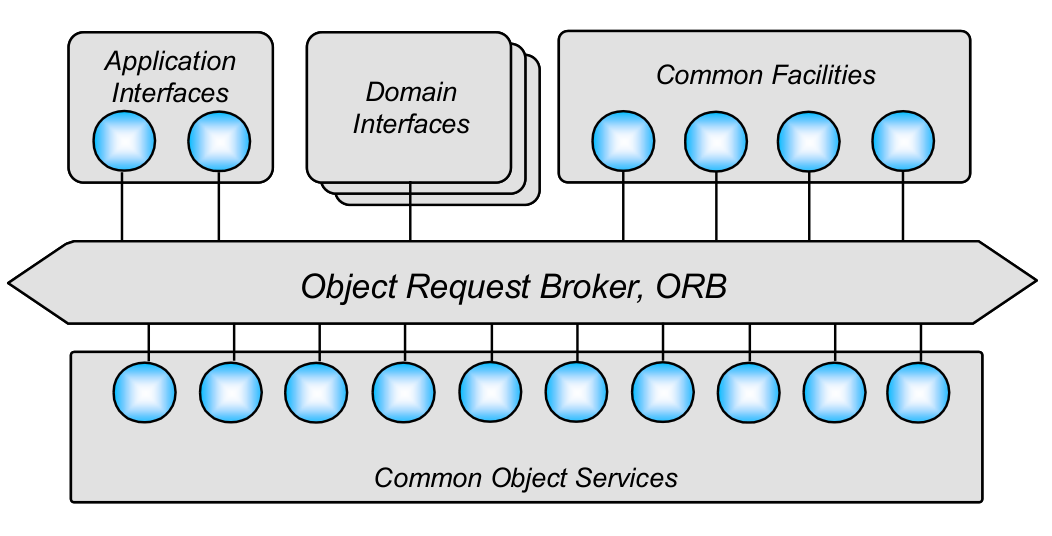
\includegraphics[width=1\textwidth]{img/OMA_Ref.png}
\caption{Esquema de funcionamiento del modelo de referencias de OMA.}
\label{OMAimg}
\end{figure}

\begin{itemize}
	\item \textit{Object Request Broker, ORB:} Bus de comunicación entre objetos.
	\item \textit{Common Object Services:} Gestión del ciclo de vida, persistencia, resolución de nombres, tiempo, control de concurrencia, seguridad...
	\item \textit{Common Facilities:} Colecciones de componentes, con funciones de tipo general, pero orientados a aplicaciones finales en vez de al sistema.
	\item \textit{Domain Interfaces:} Colección de componentes/objetos comunes específicos para áreas de aplicaciones: comercio electrónico, telecomunicaciones, banca, salud, fabricación...
	\item \textit{Application Interfaces:} Interfaces específicas de aplicaciones concretas.
\end{itemize}

\begin{defn}[ORB]
Object Request Broker → Bus de comunicación entre objetos.

Es un middleware avanzado que es la repera y permite :

\begin{itemize}
	\item Permite llamadas estáticas y dinámicas a objetos. Incluye descubrimiento dinámico de objetos.
	\item Describir las interfaces independientemente del lenguaje de programación. El lenguaje de descripción se llama \concept{IDL}\label{IDL} (Interface Description Language)
	\item Enlace directo de aplicaciones escritas en múltiples lenguajes de alto nivel (no necesariamente orientados a objetos).
	\item Sistema auto-descrito. Genera meta-información consultable dinámicamente.
	\item Soporte de seguridad,transacciones y autenticación de las comunicaciones
	\item Polimorfismo en la ejecución de funciones asociadas a un mismo mensaje.
\end{itemize}
\end{defn}

\begin{defn}[IDL]
Interface description language.
\end{defn}

Del código IDL se crean los stubs necesarios (cliente y servidor\footnote{Los stubs de servidor se llaman \textit{skeletons}}) y los ficheros de definiciones. Además, se genera código fuente del lenguaje elegido, definido en CORBA.

Este es el esquema de desarrollo de un sistema con CORBA.


\begin{figure}[hbtp]
\centering
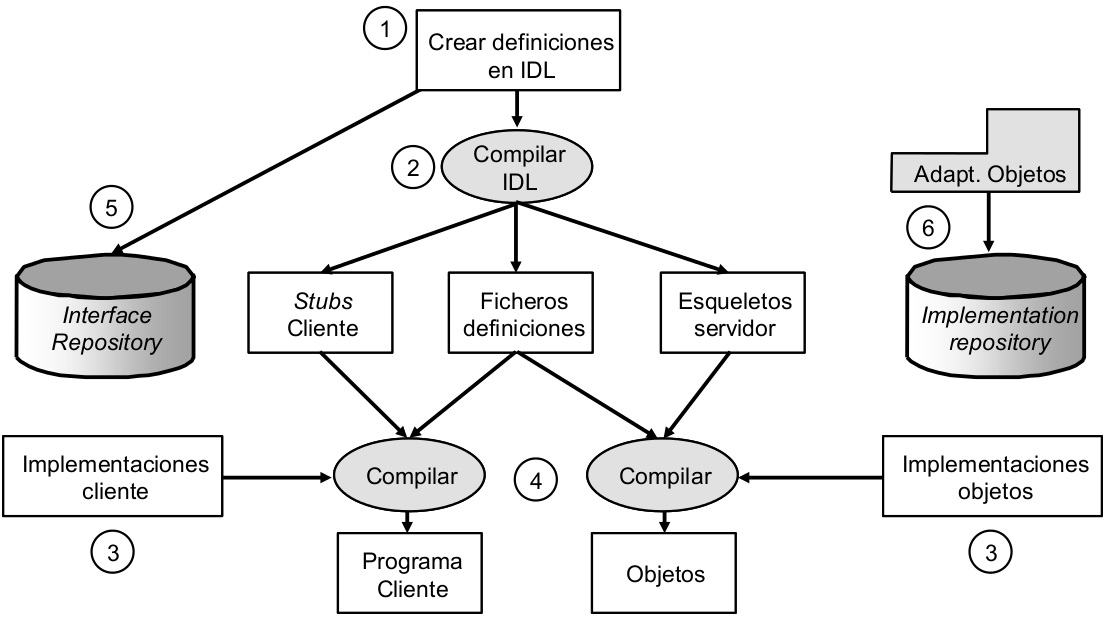
\includegraphics[width=1\textwidth]{img/CORBA.png}
\caption{Esquema del desarrollo de CORBA.}
\label{OMA}
\end{figure}


\subsubsection{Microsoft COM}

\begin{defn}[Microsoft COM]
	Microsoft Component Object Model - Plataforma de objetos de microsoft.
\end{defn}

Esta plataforma de objetos ha ido mejorandose y evolucionando a lo largo del tiempo. Primero fue \concept{DDE} (Dynamic Data Exchange) que mejoró la comunicación entre aplicaciones con \concept{OLE} (Object Linking and Embedding) hasta llegar a \textbf{COM}, con su versión de objetos distribuida \concept{DCOM} y por último, al integrarlo con MTS y MSMQ se ha llegado a \textbf{COM+}

\begin{defn}[MTS]
	Microsoft Transaction Server
\end{defn}

\begin{defn}[MSMQ]
	Microsoft Message Queueing
\end{defn}

\paragraph{Características}
Un objeto COM es un objeto en el mismo sentido que en CORBA,  es independiente del lenguaje de programación y cada objeto tiene una o varias interfaces. Estas interfaces se definen con el Lenguaje de Definición de Interfaces de Microsoft (en inglés \concept{MIDL}). Este lenguaje está basado en el IDL\ref{IDL} del \textit{Distributed Computing Environment} (\concept{DCE}) que utiliza Apollo RFC.

Los sistemas COM se organizan en componentes COM que son módulos binarios (ejecutables o librerías dinámicas). Estos módulos pueden contener uno o varios objetos COM, una interfaz gráfica e incluso otro componente\footnote{Si un componente incluye a otro, el grande se llama componente \textit{ActiveX}}

\paragraph{Funcionalidades}

\begin{itemize}
	\item Transparencia de la localización de los objetos.
	\item Activación de los objetos a distancia (a través del \concept{SCM} (\textit{Service Control Manager})
	\item Seguridad en las comunicaciones (\concept{NTLMP} (\textit{NT Lan Manager Protocol}) y \concept{SAM} (\textit{Security Access Manager})
	\item Descubrimiento dinámico de interfaces (no hay que recompilar todo cuando en un objeto se incluya una interfaz para que podamos utilizarlo)
	\item Reutilización de objetos por agregación y contenencia (\textbf{no herecia})
\end{itemize}


\subsection{Java RMI}
Vamos a ver ahora cómo implementa Java la idea de Remote Method Invocation.

Existe desde Java 1.1 y es más sencillo que CORBA. La arquitectura está basada en 3 niveles: Proxy, Referencia Remota (gestiona las referencias remotas) y Transporte (JRMP - Java remote Method Protocol). Sobre estas 3 capas se construye el cliente y el servidor. Cabe mencionar que el proxy del servidor se denomina esqueleto.

\obs No hay soporte para objetos programados en otro lenguaje (como si permitían las anteriores opciones)

Para programar con Java RMI hay que seguir los siguientes pasos:
\begin{itemize}
	\item Definir las interfaces remotas (extendiendo java.rmi.Remote)
	\item Implementar las clases remotas

	\item Crear proxy y esqueleto compilando con rmi
	\item Crear la aplicación como servidor de la clase remota
		\subitem Crear la instancia
		\subitem Se registra en el servicio de nombres.
	\item Arrancar RMIRegistry y el servidor de la clase remota.
	\item Ya podemos crear clientes con referencias remotas a objetos de la clase implementada.
\end{itemize}

\paragraph{Paso de parámetros}
\begin{itemize}
	\item Todos los parámetros son de entrada salvo el retorno del método.
	\item Admite objetos remotos como parámetros (que obviamente se pasan por referencia)
	\item Admite objetos locales como parámetros sólo si son serializables (que se pasan por valor)
\end{itemize}

\section{Servicios de directorio global}

Reflejan la composición del sistema en todo momento, gestionando el estado de los sistemas que pertenecen a él (pertenencia dinámica) y gestionando las aplicaciones que contiene cada sistema. Estos sistemas tienen que ser Cliente/Servidor para poder ser gestionados por un servicio de directorio global.

Estos servicios se encargan de resolver las transparencia con la ubicación y cada entrada tiene todos los datos asociados al elemento como el estado y la ubicación física\footnote{El servicio de directorio tiene que conocer las ubicaciones físicas y las direcciones para poder ofrecer transparencia a los sistemas que lo utilicen}, aparte de otras variables (estadísticas por ejemplo).


\subsection{Namespaces}
Estos servicios de directorio globales utilizan \concept{namespaces}, es decir, espacios de nombres, de modo que los elementos se pueden reconocer por un nombre en un directorio.

Los nombres deben ser únicos (normalmente asignados por una autoridad dentro del dominio) y no deben contener información de la localización físca, así se garantiza mejor la transparencia a la ubicación.

Este es un ejemplo de un espacio de nombres jerárquico


\begin{figure}[hbtp]
\centering
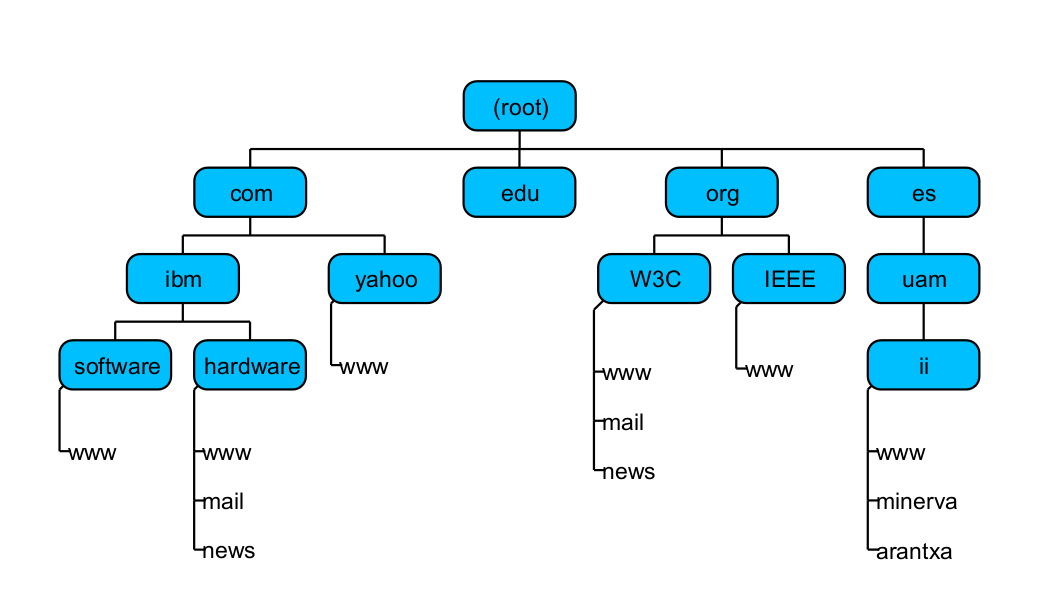
\includegraphics[width=1\textwidth]{img/namespaces.png}
\caption{Espacio de nombres jerárquico.}
\label{namespaces}
\end{figure}

Estos espacios de nombres se pueden utilizar también orientándolo a objetos, de tal manera que cada entrada es una instancia de un objeto. También se pueden tener distintas copias para cada dominio o distribuirlo organizándolo en servicios administrados separadamente ya que el acceso dentro de un dominio sólo requiere un nombre local.

\paragraph{Estándar \concept{X.500}}
Vamos a definir unas cuantas siglas\footnote{Por si acaso no llevamos ya suficientes} necesarias para explicar este estándar

\begin{defn}[XDS]
	APIs de X/Open Direcrory Service
\end{defn}

\begin{defn}[DUA]
	Directory User Agent
\end{defn}

\begin{defn}[DAP]
	Direcroty Access Protocol
\end{defn}

\begin{defn}[DSA]
	Directory System Agent
\end{defn}

\begin{defn}[DSP]
	Direcroty System Protocol
\end{defn}

Los clientes contienen el DUA y se comunicacn con los servidores utilizando DAP.

Los servidores contienen el DSA y se comunican entre servicores utilizando DSP.

Al directorio en sí se accede con las APIs de XDS.


\begin{figure}[hbtp]
\centering
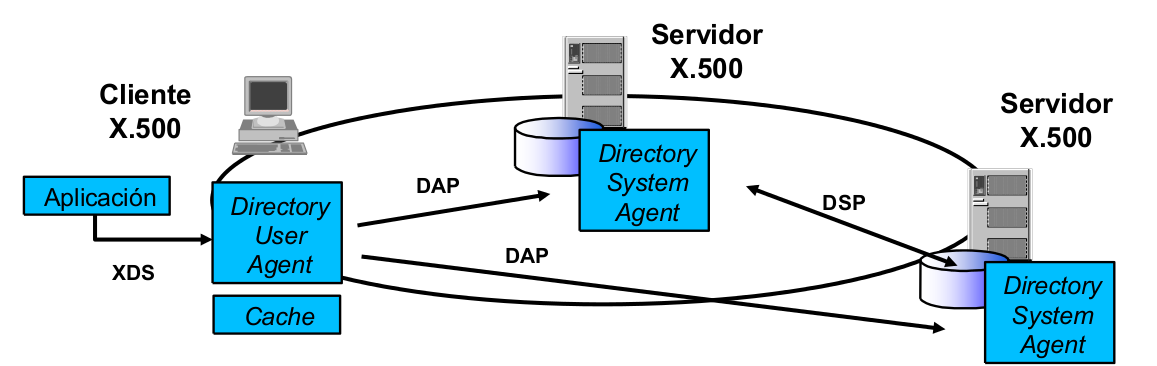
\includegraphics[width=1\textwidth]{img/X500.png}
\caption{Esquema de funcionamiento del estándar X.500.}
\label{X500}
\end{figure}

Existe una alternativa al DAP que es el \concept{LDAP} (\textit{Lightweigth Directory Access Protocol}). Este protocolo no requiere espefícicamente de un directorio X.500, puede utilizarse con \textit{Microsoft Active Directory}.

Esto es un protocolo de comunicaciones, no es una especificación de directorio ni una API de programación. No confundirse.


\subsection{Servicios de tiempo}

Es básico y fundamental que cuando tenemos un sistema distribuido todos los relojes estén perfectamente sincronizados. Para ello existen los servicios de tiempo que vamos a estudiar a continuación.

Sincronizar 2 personas sus relojes es fácil, porque los 2 ven en el mismo instante de tiempo los 2 relojes. 2 ordenadores separados no pueden ver los relojes a la vez, ya que el mensaje con la hora que tiene cada uno tarda en llegar, es por ello que cada ordenador \textbf{mantiene un componente de inexactitud} y que es necesario \textbf{sincronizar periódicamente} cuando ese componente de inexactitud supere un umbral definido\footnote{Tal vez nos podemos permitir 0.01 segundos de desincronización, pero no podemos permitirnos 0.05}

Mantener sincronizado el tiempo es imporescindible para la consistencia y para la \textbf{seguridad}.

Para lograr esta sincronización existen proveedores de tiempo (\concept{timer ticks}) que pueden sincronizar por radio      y actualizar el reloj del administrador de nuestro sistema distribuido. Podemos conectar más de un servidor a estos proveedores.

Una vez tenemos definidos los servidores de nuestro servicio con la hora buena (sincronizados con los timer ticks) el resto de nuestros servidores realizan consultas para sincronizar sus relojes. El formato utilizado es \concept{UTC} (Universal Time Coordinated) que cuenta desde el principio del calendario gregoriano.


\subsubsection{NTP}
¿Y cómo implementamos o utilizamos un servicio de tiempo? Con el \concept{NTP} \textit{Network Time Protocol}, que define una arquitectura para un servicio de tiempo y un protocolo para distribuir la información del tiempo.

\begin{itemize}
	\item Precisión en la sincronización a UTC.
	\item Fiabilidad
	\item Actualizaciones frecuentes (por lo que será necesario que sea resistente a alto nivel de carga)
\end{itemize}

La red de servidores está organizada jerárquicamente. El primer estrato recibe UTC de fuentes  físicas de tiempo (llamadas estrato 0 en wikipedia) y el estrato 2 sincroniza con los primeros. El resto de la red sincroniza con el estrato 2.

Veamos un ejemplo de los cálculos necesarios para sincronizar dos servidores.

\begin{example}
El esquema de la comunicación (intercambio de mensajes) entre los dos servidores que se van a sincronizar es:
\begin{center}
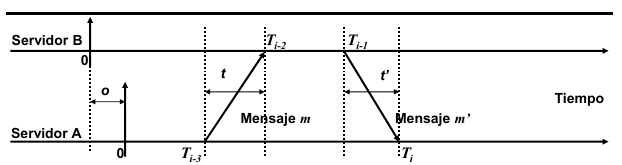
\includegraphics[width=1\textwidth]{img/ntp.png}
\end{center}

Nuestro objetivo es calcular $o$, que es la diferencia de tiempos entre ambos relojes. Observando el esquema, podemos deducir las ecuaciones:
\begin{align}
T_{i-3}+o+t=T_{i-2}\\
T_{i}+o=T_{i-1}+t'
\end{align}
Tampoco conocemos $t$ n $t'$, pues no sabemos el tiempo que ha tardado el mensaje en ser transmitido. Si sumamos las dos ecuaciones y despejamos $o$ de la nueva ecuación nos queda:
\[o=\underbrace{\frac{T_{i-2}+T_{i-1}-T_i-T_{i-3}}{2}}_{o_i}+\frac{t'-t}{2}\]

Así, tenemos $o$ escrito como la suma de un valor conocido más una desviación. Puesto que todos los tiempos son positivos, tenemos que $t+t'>t'-t$ por lo que podemos acotar $o$ mediante:
\[o_i-\frac{\overbrace{t'+t}^{d_i}}{2}\leq o \leq o_i + \frac{\overbrace{t'+t}^{d_i}}{2}\]
\end{example}

\subsection{Seguridad}
Aunque es un tema superimportante (porque en un sistema distribuido se complican las cosas) y tiene un tema dedicado explícitamente a esto, no se va a ver en este curso porque ...



\section{Problemas Tema 1}
\newpage


\chapter{Colas}
\section{Teoría}
\section{Problemas Tema 2}
% -*- root: ../SI2.tex -*-



\chapter{Aspectos operacionales de los sistemas distribuidos: Disponibilidad}
\section{Introducción}
A lo largo de este tema vamos a estudiar la teoría de la disponibilidad de los sistemas distribuídos así como algunas arquitecturas que permiten obtener un incremento de la misma.

Para empezar debemos definir qué es la disponibilidad.

\begin{defn}[Disponibilidad]
La disponibilidad de un sistema es la probabilidad de que este se encuentre operativo en un instante de tiempo determinado.
\end{defn}

Hay dos motivos por los que un sistema puede no estar disponible:
\begin{enumerate}
\item[1] \textbf{Paradas no planificadas}

Este tipo de paradas se deben a fallos en los equipos o en los programas que implementan los servicios.

Requieren tratamiento estadístico, pues no habrá dos iguales. Los sistemas que las minimizan se llaman de \textbf{Alta Disponibilidad} \textit{(High Availability, HA)}


Algunas de las causas más frecuentes por las que se producen este tipo de paradas son:

\begin{itemize}
\item Extensión del tiempo destinado a operaciones planificadas.
\item Error humano.
\item Fallo en aplicación.
\item Fallo del sistema operativo.
\item Fallo hardware.
\item Errores de configuración del software.
\end{itemize}

\item[2] \textbf{Paradas planificadas}

Son requeridas por la aplicación para su correcto funcionamiento: Rearranques programados, copias de seguridad, cambios de configuración...

Por ser previsibles permiten un tratamiento sistemático. Los sistemas que las minimizan se denominan de \textbf{Operación Continua} \textit{(Continuous Operation, CO)}

Algunas de las causas más frecuentes por las que se producen este tipo de paradas son:

\begin{itemize}
\item Copias de seguridad.
\item Reemplazar o actualizar hardware.
\item Reemplazar o actualizar aplicaciones.
\item Actualizar sistema operativo.
\item Instalación de parches
\end{itemize}
\end{enumerate}

Evidentemente, un sistema ideal sería de Alta Disponibilidad y de Operación Continua. No obstante, a mayor disponibilidad del sistema mayor es el coste del mismo y su mantenimiento. Por tanto, es necesario valorar el nivel de disponibilidad requerido para un funcionamiento aceptable e invertir lo necesario para conseguirlo sin tratar de superarlo.

Antes de seguir estudiando el tema de la disponibilidad, vamos a ver una serie de definiciones de términos que aparecerán a lo largo de los apuntes y que es necesario precisar.

\begin{defn}[Fiabilidad (Reliability)][Fiabilidad]\index{Reliability}
Probabilidad de que un componente o sistema continúe funcionando en un determinado instante en el tiempo.
\end{defn}

\begin{defn}[Elasticidad o Resiliencia (Resiliency)][Resiliencia]\index{Elasticidad}\index{Resiliency}
Capacidad de un sistema para adaptarse a
condiciones externas imprevistas (fallos, aumento de carga...) para continuar cumpliendo sus parámetros de calidad.
\end{defn}

\begin{defn}[Mantenibilidad (Serviceability)][Mantenibilidad]\index{Serviceability}
Es la probabilidad de realizar una reparación satisfactoria en un tiempo determinado.
\end{defn}

\begin{defn}[Sistemas\IS tolerantes a fallos (Fault-Tolerant Systems)][Sistemas\IS tolerantes a fallos]
Sistemas que contienen
componentes hardware dobles de modo que el fallo de uno de ellos no suspende su
operación.
\end{defn}
\newpage
\begin{defn}[Clusters\IS de alta disponibilidad (High Availability Clusters)][Clusters\IS de alta disponibilidad]
Conjunto de nodos de servicio que comparten conexiones externas (red, discos...) y están gestionados por un software especial que permite proporcionar servicio sin interrupciones ante el fallo de alguno de sus componentes.
\end{defn}

\begin{defn}[Clusters\IS de alto rendimiento (High Performance Clusters)][Clusters\IS de alto rendimiento]
Conjunto de nodos de servicio que comparten una misma carga de trabajo.
\end{defn}

\begin{defn}[Recuperación ante desastres (Disaster Recovery)][Recuperación\IS ante desastres]
Capacidad de una instalación de
recuperar la operatividad tras un evento de gran magnitud, bien de tipo local (edificio), urbano (ciudad) o regional (área extendida con infraestructuras comunes).
\end{defn}

\section{Teoría de la disponibilidad}
\subsection{Disponibilidad}
La disponibilidad, $A$, de un sistema se estima a partir de la medida del tiempo que ha estado operativo, $T_{op}$, en un intervalo de tiempo, $T_{tot}$, suficientemente grande.
\[A= \frac{T_{op}}{T_{tot}}\]

Pero esta medida no da una idea global de la disponibilidad del sistema, pues un mismo valor puede obtenerse de la misma forma.

Por ejemplo, no es lo mismo que un sistema esté disponible 99 horas de cada 100 que 99 segundos de cada 100. Incluso si dos datos se han obtenido dividiendo los datos en las mismas unidades y estamos, por ejemplo, en 99 horas de cada 100 de actividad, puede ser que el sistema haya fallado una única vez en esas 99 horas y tardase una hora en recuperarse o que el sistema falle cada media hora tardando poco en recuperarse.

Por ello se utilizan otras medidas para estudiar la disponibilidad del sistema.

\begin{defn}[Tiempo medio\IS entre fallos]

En inglés \textbf{Mean Time Between Failures, MTBF}, es valor esperado del tiempo que transcurre entre dos fallos consecutivos de un equipo.
\end{defn}

\begin{defn}[Tiempo medio\IS hasta el fallo]

En inglés \textbf{Mean Time To Failure, MTTF}, es el valor esperado del tiempo de vida de un equipo o sistema, medida de su Fiabilidad (Reliability).
\end{defn}

\begin{defn}[Tiempo medio\IS de reparación/recuperación]

En inglés \textbf{Mean Time To Repair/Restore, MTTR}, es el valor esperado del tiempo que se tarda en sustituir un equipo averiado o recuperar un fallo de software.
\end{defn}

A partir de estos valores se calcula la disponibilidad según la fórmula:

\[A=\frac{MTTF}{MTBF}=\frac{MTTF}{MTTF+MTTR}\]

Para pasar de la primera a la segunda fórmula se emplea la relación lógica $MTBF=MTTF+MTTR$, es decir, el tiempo que transcurre entre dos fallos es la suma del tiempo que tarda en recuperarse el sistema tras un fallo más el tiempo que tarda en volver a fallar.

\subsection{Fiabilidad}

La fiabilidad de un componente o sistema en el tiempo es la probabilidad de que el sistema continúe funcionando en un instante de tiempo. Si denominamos $T$ al tiempo de vida del componente, su fiabilidad viene dada por la expresión:
\[R(t)=\mathbb{P}\{T > t \}\]

La vida del componente, $T$, es una variable aleatoria, cuya función de distribución es
\[F_T(t)=\mathbb{P}\{T \leq t \}\]

Evidentemente ambas variables probabilidades deben sumar siempre 1, $R(t)+F_T(t)=1$ y derivando obtenemos que sus funciones de densidad son iguales pero de signo contrario.

Una vez hemos definido estas variables podemos definir el tiempo medio hasta fallo como la esperanza de vida de un componente:
\[MTTF = E[T]=\int_{-\infty}^{\infty}fF'_T(t)dt\]

Ahora, sabiendo algo de probabilidad, podemos calcular la probabilidad de que un sistema falle antes de un instante, $x$, sabiendo que funcionaba en un instante $t<x$.
\[F_T(x | T > t ) = \mathbb{P}\{T \leq x | T> t\}=\frac{\mathbb{P}\{(T \leq x) \cap (T > t)\}}{\mathbb{P}\{T > t\}}=\frac{\mathbb{P}\{t < T \leq x\}}{\mathbb{P}\{T > t\}}=\]
\[=\frac{F_T(x)-F_T(t)}{1-F_T(t)}\]

y derivando con respecto a $x$ se obtiene
\[f_T(x | T > t)=\frac{f_T(x)}{1-F_T(x)}\]

A partir de esta última expresión se define la \concept{función de tasa de fallo} al evaluarla en $x=t$.
\[r(t)=f_T(t | T > t)=\frac{-R'(t)}{R(t)}\]

y se interpreta como la probabilidad de que un componente que funciona falle en el instante siguiente:
\[\mathbb{P}\{t<T\leq t + dt | T > t\}=f_T(t | T > t)dt=r(t)dt\]

Si la tasa de fallos tiene un valor constante, integrando la función $r(t)$ entre $0$ y $t$ y despejando $R(t)$ llegamos a:
\[R(t)=e^{-λt} \implies F_T(t) = 1-e^{-λt}\]

con lo que acabamos de obtener que el tiempo de vida es una distribución exponencial y su valor esperado será el MTTF=1/λ

\subsection{Distribución de los fallos}

La función de tasa de fallos en un equipo tiene la forma que se muestra en la figura:
\begin{center}
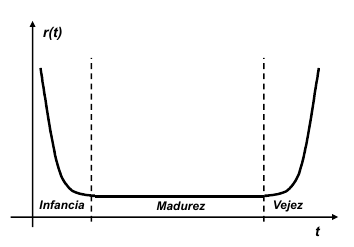
\includegraphics[width=0.7\linewidth]{img/tasa_fallos.png}
\end{center}

Durante la zona de infancia la tasa de fallos es alta debido al montaje de componentes defectuosos. Esta tasa de fallos se reduce con el tiempo hasta alcanzar una etapa de madurez que se correspondería con la época en que tenemos tasa de fallos constante. Por último el envejecimiento del equipo aumenta la tasa de fallos.

Todos los cálculos se realizan pensando en la zona de madurez del equipo, trabajando con $r(t)=cte$

Por otro lado tenemos también los fallos en programas que pueden dividirse en dos tipos según su tratamiento
\begin{enumerate}
\item[1] Programas que no son reparados cuando se encuentra el fallo sino que es necesario esperar a que se publique una nueva versión del mismo. Es la situación habitual en producción y con programas cerrados.

El modelo de tasa de fallos constante es válido durante el uso de una misma versión. Al cambiarla es necesario recalcular todos los datos.

\item[2] Programas cuyos defectos se corrigen conforme se encuentran. Suele tratarse de programas de producción propia o ciclos de pruebas en la producción de programas. El principal problema es que la solución de un defecto puede y suele introducir otros nuevos.

En este caso el modelo de tasa de fallos constante no es válido ya que tendremos una tasa de fallos que decrece con el tiempo (según se van arreglando los desperfectos). Su forma depende del modelo elegido para el ritmo de descubrimiento de fallos.

\end{enumerate}

\subsection{Mantenibilidad}
Es la probabilidad de realizar una reparación satisfactoria en un tiempo determinado. Mide la rapidez y facilidad con que un sistema se vuelve a poner operativo tras un fallo.
\[M(t)=\mathbb{P}\{T'> t\} \text{ con T' el tiempo de reparación}\]

Este tiempo incluye el tiempo necesario para descubrir el fallo, encontrar la causa, conseguir las piezas necesarias, la instalación de las mismas, arrancar el sistema de nuevo, etc. Es decir, incluye todo el tiempo gastado desde que \textbf{se produce} el fallo (aún si no se detecta) hasta que se resuelve el problema.

\[MTTR=E[T']\]

\subsection{Componentes en serie vs Componentes en paralelo}

Si tenemos un sistema compuesto por componentes en serie, un fallo en cualquiera de ellos implica un fallo global. La conexión en serie puede no ser física pero si lógica, una componente depende del resultado del trabajo de otra.

Suponiendo que el fallo en cada componente es independiende del resto, tenemos:
\[A= \prod_{i=1}^{n}A_i; \ \ \; R(t)=\prod_{i=1}^{n}R_i(t); \  \ \; r(t)=\sum_{i=1}^{n}r_i(t)\footnote{No veo clara esta fórmula}\]

Si tenemos un sistema compuesto por componentes en paralelo y estas componentes son redundantes para su funcionamiento, un fallo en una de ellas no implicará un fallo en el sistema.

Suponiendo que el fallo en cada componente es independiente nos queda:
\[A= 1-\prod_{i=1}^{n}(1-A_i)\footnote{Estará disponible cuando al menos una componente esté disponible}; \ \ \; F_T(t)=\prod_{i=1}^{n}F_{T_i}(t); \  \ \; R(t)= 1-\prod_{i=1}^{n}(1-R_i(t))\]

\begin{center}
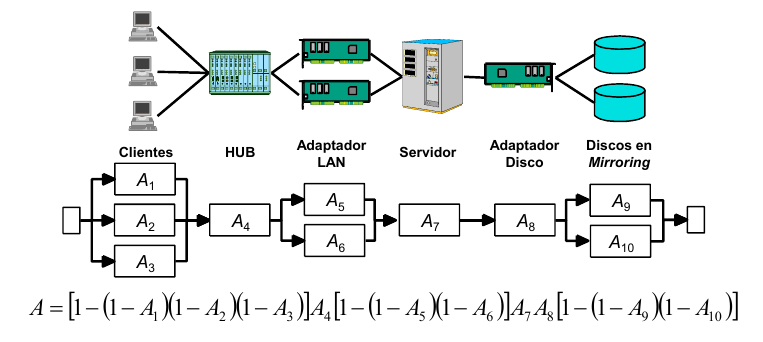
\includegraphics[width=\linewidth]{img/disponibilidad.png}
\end{center}



\section{Mejoras de la disponibilidad}

Recordemos la ecuación inicial que dimos para la disponibilidad:
\[A=\frac{MTTF}{MTTF+MTTR}=\frac{1}{1+MTTR/MTTF}\]

simplemente viendo esta fracción podemos ver que la disponibilidad de un sistema puede mejorarse (aumentar) de dos formas:
\begin{itemize}
\item Aumentando $MTTF$ mejorando la calidad de los equipos, introduciendo redundancias o eliminando \textbf{Puntos Simples de Fallo}

\item Reduciendo $MTTR$ mediante la reducción del tiempo empleado en cualquiera de las siguientes fases:
\begin{itemize}
\item Tiempo de \textbf{latencia} (desde que se da el fallo hasta que se descubre que algo falla)

\item Tiempo para aislarla (desde que se descubre hasta que se encuentra el motivo)

\item Tiempo para corregirla

\item Tiempo para verificar que todo funciona bien
\end{itemize}
\end{itemize}

\subsection{Arquitecturas que incrementan la disponibilidad}

La disponibilidad de una cadena de procesamiento es siempre menor que la menor de las disponibilidades de sus componentes. Denominamos \concept{Single Point Of Failure, SPOF} a los puntos más criticos del sistema, aquellos que al fallar implican la caída del servicio.

Como es evidente, la forma en que más podemos incrementar el $MTTF$ de cada componente es mediante la creación de un \textbf{cluster} (elementos redundantes) en cada parte de la cadena de procesamiento. Esta solución, además, elimina los SPOF al añadir redundancias incluso a esos componentes más críticos.

Conseguir que varios sistemas realicen en paralelo una misma función no es sencillo y la solución empleada depende de factores como el tipo de elemento al que se le quiere dar redundancia y las necesidades de disponibilidad del sistema completo.

En cualquier caso, siempre es necesario considerar dos procesos a la hora de implementar un sistema: el cómo actuar cuando se produce un fallo para poder mantener el servicio, \concept{Fail-over}, y cómo actuar para recuperar la situación normal una vez se resuelve el fallo \concept{Fail-back}.

Existen diferentes tipos de redundancia:
\begin{enumerate}
\item[1] \textbf{Según el estado de cada elemento del cluster}

Pueden estar todos los elementos activos (AA), uno activo y el resto preparados para activarse casi instantáneamente (AS) o uno activo y el resto detenidos pudiendo activarse en un cierto periodo de tiempo (AP)

\item[2] \textbf{Según el reparto de carga entre los elementos del cluster}

Puede ser dinámico (D), en cuyo caso no habrá que preocuparse en caso de fallo de un componente; o estático (E), donde un fallo implica reconfigurar el reparto de carga

\item[3] \textbf{Según el tratamiento de las conexiones activas}

Las sesiones activas pueden continuar (C) tras un fallo o ser interrumpidas (I).
\end{enumerate}

\section{Redundancia en los sistemas de comunicaciones}
Los sistemas de comunicaciones son uno de los puntos críticos de todo sistema distribuido.

Vamos a distinguir la redundancia en las redes de área local (LAN) y en redes de área extendida (WAN) considerando en ambos casos los estándares de facto actuales: redes LAN basadas en Ethernet y TCP/IP como medio de transporte.

Las características de los equipos que actualmente se emplean para implementar una LAN hacen que estas redes se puedan construir atendiendo a tres modelos distintos:
\begin{itemize}
\item \textbf{Nivel 2 compartido} Múltiples servidores se conectan a un mismo segmento de LAN implementado en un \textit{Hub}. Es el menos utilizado por ser el menos eficiente y flexible.

El hub es un dispositivo que tiene la función de interconectar las computadoras de una red local. Su funcionamiento es más simple comparado con el Switch y el router:
El hub recibe datos procedentes de una computadora, los transmite a los demás. En el momento en que esto ocurre, ninguna otra conmutadora puede enviar una señal. Su liberación surge después que la señal anterior haya sido completamente distribuida.


\item \textbf{Nivel 2 conmutado} Cada enlace es un segmento de LAN. Todos los componentes se interconectan mediante \textit{switches}, que actúan como puentes multipuerta.

Suele emplearse en el \textbf{nivel de acceso}, por ejemplo, en las conexiones de los ordenadores de las granjas de servidores.

\item \textbf{Nivel 3} Cada enlace es un segmento de red que une un elemento con un \textit{router}. El \textit{router} se implementa también en los propios \textit{switches} mediante módulos especiales.

Suele emplearse en el \textbf{nivel de agregación} interconectando diversos niveles de acceso, servidores especiales y redes externas.
\end{itemize}

Estos modelos suelen coexistir dentro de un Centro de Proceso de Datos (CPD)
\begin{center}
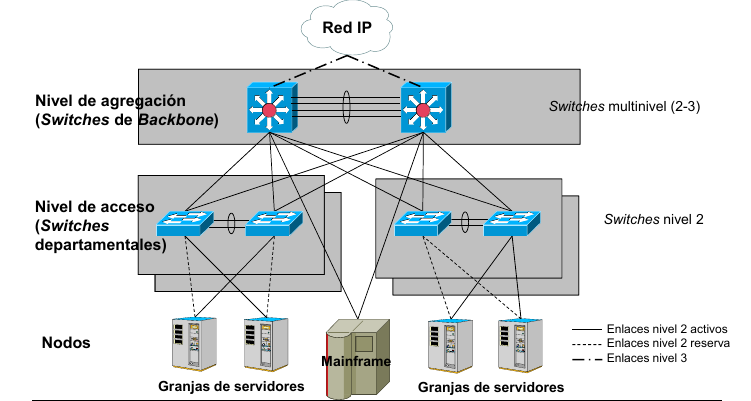
\includegraphics[width=\linewidth]{img/niveles.png}
\end{center}

La instalación de redundancias en el nivel 3 implica el uso de un protocolo de encadenamiento dinámico (OSPF, BGP), igual que en el caso de redes de área extendida (WAN).

A nivel 2, implica la aparición de bucles en los posibles caminos entre dos nodos de la red lo que lo hace incompatible con el protocolo \textit{Transparent Bridging} empleado en Ethernet. Este problema se resuelve con el \textit{Spanning Tree Protocol}, que se mejoró con el \textit{Rapid Spanning Tree Protocol}. Para optimizar el uso de VLANs se deben crear múltiples \textit{spanning trees}, solución proporcionada por \textit{Multiple Spanning Tree}.

En definitiva, si en la red de comunicación tenemos redundancias en un determinado nivel, es necesario emplear un protocolo que permita encontrar el mejor camino de un elemento a otro aún con las redundancias.

\subsection{Rapid Spanning Tree Protocol, RSTP}

Al aplicar este protocolo tenemos cada switch asociado a un identificador que nos da su prioridad. El de mayor prioridad (menor identificador, ID1) se denomina switch raíz. El siguiente en prioridad se le denomina switch raíz alternativo (ID2).

Para cada puerto hay que determinar de que tipo es:
\begin{itemize}
\item Raíz. Da el mejor camino al switch raíz

\item Designado. Proporciona a cada segmento de red conectado al switch el mejor camino al switch raíz. Es decir, que para algún nodo, su mejor camino hasta el nodo raíz implicar coger justo este enlace.

\item Alternativo. Otros.
\end{itemize}

Periódicamente, cada switch genera una \textit{Bridge Protocol Data Unit, BDPU} y la envía a todos los switches de la red.

\textcolor{red}{Mirar el ejemplo de moodle subido por la profesora. Explica bastante bien el protocolo}

\subsection{Detección de fallos en RSTP}
Puede producirse un fallo en un enlace conectado a un RP o DP, que se detecta directamente por los switches que forman el enlace; o puede darse un fallo en un switch. Si hay tres turnos seguidos en los que no se recibe BDPU de un switch, se le da por muerto.

Tras el fallo, todos los switches reconfiguran el spanning tree, mediante intercambios locales de los switches afectados por el cambio y el resultado se propaga al resto de la red.

\obs Hay otra versión de este mecanismo es el \textit{spanning tree normal}, en el que únicamente el root bridge transmite BPDU. Sólo se detecta un problema tras 20 segundos (vida máxima) y tras esto recalculamos el spanning tree completo.

\subsection{Redundancia en la conexión de servidores a nivel 2}
La redundancia básica en la conexión de un ordenador a una LAN se consigue mediante el uso de dos o más adaptadores de red.

Los puertos de estos adaptadores (un puerto por adaptador) tendrán la misma MAC, pero sólo uno de los adaptadores estará disponible. Si cae, el sistema activará otro. No afecta a los protocolos de niveles superiores.

\begin{defn}[EtherChannels]
Consiste en la agrupación de enlaces Ethernet donde todos los puertos poseen la misma MAC como si fuesen sólo 1 (y así lo ven desde arriba) y están activos simultáneamente.

Da mayor rapidez en la resolución de fallos y mejora el ancho de banda pero su implementación es costosa. Se requiere que ambos extremos de la conexión tengan soporte de \textbf{EtherChannels}. Los componentes de un \textbf{EtherChannel} no se pueden disgregar para conectar varios dispositivos distintos. A todos los efectos, es un único enlace.

\end{defn}

\subsection{Redundancia de las WAN}
Las redes WAN permiten establecer la interconexión entre elementos distantes de sistemas distribuídos. Se basan en el protocolo TCP/IP y se distinguen dos tipos de componenetes: enlaces y unidades de encadenamiento (routers).

La alta disponibilidad de las WAN se consigue teniendo muchos routers y enlaces para que siempre haya caminos alternativos. La gestión del tráfico a través de las diferentes rutas se lleva a cabo con los protocolos de encadenamiento dinámico que estudiamos en Redes: OSPB y BGP.

\begin{defn}[OSPF]
Protocolo de encadenamiento dinámico eficaz y ampliamente utilizado en redes IP. Se basa en el conocimiento de toda la red y el empleo de Dijkstra para localizar el camino más corto. Se organiza la red en áreas dentro de las cuales los routers encaminan los paquetes. Para cambiar de área se emplean los Area Border Gateways (routers fronterizos)

El mensaje OSPF Hello se emplea para conocer la topología de la red con lo que cada router conoce a sus vecinos. Y con el mensaje Link State se informa del estado de los enlaces.
\end{defn}

Se puede producir un fallo en OSPF por la caída de un enlace, que se deteca de forma inmediata, por la caída de un router, que se detecta gracias al protocolo OSPF Hello, que sirve de \textit{keep-alive}. El mensaje Hello se intercambia cada 10 segundos. Si tras cuatro rondas no se han recibido Hello's de un router, se le da por muerto.

Si en un caso concreto se requiere una configuración estática (estaciones de trabajo, por ejemplo) el router por defecto que se asigna a estos dispositivos se convierte en un SPOF (Single Point Of Failure). Para evitarlo se emplea un cluster de routers controlado con el protocolo \textit{Virtual Router Redundancy Protocolo, VRRP}

\begin{defn}[VRRP]
Protocolo de \textit{clustering} para routers empleado para proporcionar redundancia en routers en los casos en que representan un punto único de fallo en rutas de la red. El router se sustituye por un \textit{virtual router} formado por un router activo y otro en \textit{stand-by}.

El router de mayor prioridad será el activo y asume como propias una dirección IP y una MAC que habrán sido asignadas al router virtual. Si cae el router se activa otro.
\end{defn}

El router activo envía mensajes Hello en \textit{multicast} cada x segundos. Si transcurre un tiempo predefinido sin recibir mensajes Hello se da al router por muerto y se activa el siguiente en prioridad. Este tiempo de espera predefinido es menor cuanto menor sea la prioridad. Así cuando esté un router activo que no sea el inicial, tendrá más probabilidades de que se le de por muerto, por lo que el router principal tendrá más probabilidades de volver.

En el \textbf{fail-back} hay dos opciones:
\begin{itemize}
\item Si la configuración activa preempt, el router de mayor prioridad asume el tráfico. Supone una breve interrupción del servicio mientras se produce el cambio.
\item Si la configuración desactiva preempt, se deja el router actual como activo hasta un posible fallo, quedando el reincorporado como router de backup.
\end{itemize}

\begin{defn}[Balanceador de carga]
Un balanceador de carga es un dispositivo capaz de distribuir peticiones entre un grupo de servidores para su proceso. Tiene como objeto aumentar la capacidad de proceso y la disponibilidad del servicio.

Previamente se realizaba este proceso en redes IP a través del DNS, resolviendo el mismo nombre por distintas IP pero esto no garantizaba que el servidor estuviera activo y los cambios del DNS son lentos al propagarse por la red.

Frente a un switch que sólo maneja información de nivel 2 y un router que sólo maneja información a nivel 3, el \textbf{Load Balancer, LB} también utiliza información de los niveles de transporte y aplicación para realizar el encadenamiento. Como mínimo debe garantizar que en TCP todos los paquetes de la misma conexión van al mismo servidor.
\end{defn}

Para emplear un LB, se asigna una dirección IP virtual (VIP), puerto y protocolo para el servicio a prestar; se asocian al LB los servidores que prestan el servicio y se definen unos mecanismos de distribución de carga y entrega de paquetes.

Cuando llega una petición, el LB decide qué servidor debe atenderla y se la reenvía. El servidor procesará la petición y devolverá una respuesta que será reenviada al cliente. Este último paso, según la configuración de entrega de paquetes, puede eliminarse siendo el servidor quien directamente responde al cliente. (Direct Server Return vs Destination NAT)

El mecanismo de distribución de carga puede ser cualquiera: Round Robin, alterno, menor número de conexiones, ponderado, mejor tiempo de respuesta, por origen de la petición, etc.

En cualquier caso es necesario considerar condiciones límite para realizar la entrega:
\begin{itemize}
\item Máximo número de conexiones permitido
\item Umbral de tiempo de respuesta
\item \textbf{Gracefull Shutdown}. No mandar más mensajes a un servidor que quiere desconectarse
\item \textbf{Tiempo de gracia}. Tiempo que se deja a un servidor desde que está activo hasta que se le envía tráfico, para permitir su estabilización adecuada.
\end{itemize}

Si todos los paquetes de respuestas pasaban por el LB, se puede detectar un fallo si un servidor deja de responder, se puede monitorizar en \textit{handshake} de TCP o los códigos de retorno de HTTP. Si no es así, se emplean pruebas de nivel 3 con ICMP echo/replay; a nivel 4, con apertura/cierre de conexiones TCP; o pruebas de nivel 7, tratar de conectar con la aplicación. Estos acciones las realizaría el LB para comprobar que el servidor esté activo.

El LB debe ser capaz de hacer que un cliente se conecte siempre a un mismo servidor para que se mantenga la sesión, que no está implementada de modo estándar en TCP/IP. Existen diferentes formas de hacerlo:
\begin{itemize}
\item Aplicando un algoritmo de balanceo por origen. Tiene el problema de que si varios clientes están tras una NAT son indistinguibles en este sentido.
\item Por concurrencia de conexiones. Una nueva petición de un cliente se envía al mismo servidor que mantiene la actual
\item Cookies o identificadors SSL que guarden información de la sesión. Requiere analizar el paquete e impide que el balanceo se haga por paquete. Es necesario partir la conexión TCP en el LB
\end{itemize}

\subsection{Redundancia en los sistemas de almacenamiento de la información}
La información es el punto más crítico de todo sistema informático puesto que perder datos o no tenerlos disponibles adecuadamente puede ser fatal para cualquier tipo de negocio.

La redundancia de este tipo de elementos es más compleja pues es necesario mantener la consistencia y garantizar que los elementos de procesamiento redundantes accedan a la misma copia de la información.

Existen diferentes arquitecturas de almacenamiento. Veamos algunas:
\begin{itemize}
\item \textbf{Conexión direta (Direct Attached Storage, DAS)}. Consiste en conectar el dispositivo de almacenamiento directamente al servidor o estación de trabajo, es decir, físicamente conectado al dispositivo que hace uso de él. Normalmente se usa directamente el protocolo SCSI en alguna de sus variantes.

\item \textbf{Conexión a red (Network Attached Storage, NAS)}. Es el nombre dado a una tecnología de almacenamiento dedicada a compartir la capacidad de almacenamiento de un computador (Servidor) con computadoras personales o servidores clientes a través de una red (normalmente TCP/IP), haciendo uso de un Sistema Operativo optimizado para dar acceso con los protocolos CIFS, NFS, FTP o TFTP.

\item \textbf{Red de área de almacenamiento (Storage Area Network, SAN)}. Red dedicada al almacenamiento que está conectada a las redes de comunicación de una compañía. Además de contar con interfaces de red tradicionales, los equipos con acceso a la SAN tienen una interfaz de red específica que se conecta a la SAN. Utiliza fibra óptica como medio de transporte y el protocolo \textit{FibreChannel}

\item \textbf{Internet SCSI (iSCSI)} Estándar que permite el uso del protocolo SCSI sobre redes TCP/IP

\item \textbf{FibreChannel Over IP (FCIP)} Encapsula el protocolo FibreChannel sobre IP estableciendo túneles FC sobre TCP.

\item \textbf{Internet Fibre Channel Protocol (iFCP)} Implementa FC sobre IP pero no en modo túnel sino interpretando el protocolo FC.
\end{itemize}

Uno de los métodos para mantener redundante la información en unos ciertos discos es el uso de \textbf{Redundan Array of Independen Disks, RAID}, que ya hemos estudiado en otras asignaturas.

\begin{center}
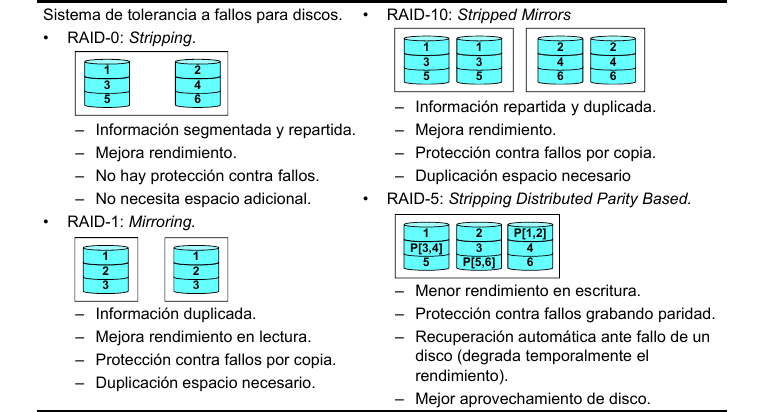
\includegraphics[width=\linewidth]{img/raid.png}
\end{center}

Los servidores de disco proporcionan herramientas autónomas para garantizar la copia de la información, y garantizar así su disponibilidad para los servidores que la utilizan, liberando así a los servidores de aplicaciones de la tarea de realización de las copias.

Estas copias pueden ser locales o remotas. Estas últimas podrían ser síncronas o asíncronas.

Dentro de las copias locales existen dos tipos: clonación de discos (se copia la información de una Unidad Lógica\footnote{Viene a ser como las particiones lógicas pero que afectan a diferentes discos, no sólo a 1} a otra) y las copias instantáneas (\textit{Snapshots o Flash Copy}).

\begin{defn}[Flash Copy]
Copia de una Unidad Lógica en el instante que se solicita, copiando los punteros a los sectores que contienen la información.

En caso de que haya una actualización de un sector, se copia la información antigua y se actuliza el puntero de la copia instantánea.

Se emplean para generar una copia consistente de la información en un momento preciso para su uso posterior.

\obs Básicamente guardas un puntero a la posición guardada. Si no la modifican, pues ya lo tienes. Si se modifica esa parte del disco, mueves la antigua información a otro sitio y actualizas tu puntero.
\end{defn}

Las copias remotas \textbf{síncronas} consisten en que la actualización de la información del servidor primario se copia a los secundarios y el proceso no finaliza hasta que no se ha actualizado la información en todos los servidores, lo que da lugar a una alta latencia de escritura. \textbf{Empleado para realizar copias locales que garanticen la alta disponibilidad}

En las \textbf{asíncronas}, una vez se actualiza el primario se guardan los cambios en un buffer y se van aplicando en el resto de servidores mediante un proceso en paralelo. Requiere un protocolo de sincronización. \textbf{Empleado para realizar copias remotas que permitan la recuperación ante desastres} \href{http://searchdatacenter.techtarget.com/es/consejo/Ventajas-e-inconvenientes-de-la-replicacion-remota-en-la-recuperacion-de-desastres}{Leer más}

Las posibles averías en discos físicos individuales son resueltas por la arquitectura RAID. Si se producen averías en una Unidad Lógica (LUN) completa o en un servidor de disco se siguen los siguientes pasos:
\begin{enumerate}
\item[1] \textbf{Fail-Over}. Se interrumpe la copia remota y la LUN secundaria pasa a principal. Para ello se notifica al servidor de proceso que debe usar a LUN secundaria y se comienza a registrar los cambios.

\item[2] \textbf{Fail-Back} Se copia el secundario activo al primario una vez recuperado. Para ello se detiene el trabajo del servidor de proceso, se reestablece la copia y se notifica al servidor de proceso que puede seguir utilizando el primario.
\end{enumerate}


\subsection{Redundancia en los sistemas de proceso}
Este tipo de redundancia se consigue mediante la asociación de los elementos de proceso (servidores) en grupos (clusters) que realizan una tarea común.

Cada servidor ejecutará un determinado número de grupos de servicio compuesto por una identidad de red (direcciones a las que el servicio responde), un conjunto de información almacenada en discos físicos o LUNs y un conjunto de procesos.

Si un servidor de un cluster falla, los grupos de servicio que soporta deben ser trasladados a otro elemento del cluster.

Básicamente un grupo de servicios es un conjunto de actividades que desempeña un servidor, es decir, procesos que ejecuta, direcciones a las que responde y memoria que usa. Si el servidor cae y no puede desempeñar estas actividades, otro tiene que ocupar su lugar.

Hay tres tipos de clusters según su modo de funcionamiento y gestión.
\begin{enumerate}
\item[1] \textbf{Clusters Activo-Pasivo o asimétricos:} Cada grupo de servicio se ejecuta en un nodo. Existen nodos de reserva en stand-by para ejecutarlos en caso de fallo.

\begin{defn}[Heartbeat]
In computer clusters, heartbeat network is a private network which is shared only by the cluster nodes, and is not accessible from outside the cluster. It is used by cluster nodes in order to monitor each node's status and communicate with each other.

Es uno de los puntos críticos de un \textit{cluster} de alta disponibilidad. Si falla se producirá la activación simultánea de ambos nodos, generando conflicos y caída del servicio.

Puede implementarse como una red de área local o mediante la escritura en una sección reservada de disco compartido.
\end{defn}

Para aumentar la fiablidiad del \textbf{heartbeat} se pueden tomar diversas medidas:
\begin{itemize}
\item Eliminar SPOF en los mecanismos de transporte del heartbeat.
\item Emplear dos heartbeat (dos redes o red+disco). Actuar sólo en caso de fallo
de ambos.
\item Emplear redes independientes lo más simples posibles: cable cruzado para
dos nodos, o segmentos de LAN con switches independientes.
\item Vigilar el correcto funcionamiento de los procesos que generan y atienden los
hearbeats en cada nodo. Instalar un watchdog local que los rearranque en caso de caída.
\end{itemize}

Existe una serie de \textbf{problemas a la hora de rearrancar en el servidor secundario} en el caso de fallo de uno de los nodos.

Si el cambio en la dirección IP se realiza sobre un adaptador con otra dirección MAC, la caché ARP de los clientes mantendrá la antigua hasta que detecten la nueva situación. Por ello se asume también la antigua dirección MAC.

Cuando la parada es no planificada (se dió un fallo en el sistema) se perderán datos de las aplicaciones, las cachés de disco y/o transacciones que se estuvieran realizando. Es por ello que el arranque de servicios en el servidor de reserva se hace siguiente los procedimientos de arranque tras un cierre anormal:
\begin{itemize}
\item Revisión de la consistencia de los sistemas de archivos a nivel de sistema operativo.
\item Revisión de la consistencia de los datos en disco a nivel de aplicación (por ejemplo, bases de datos).
\item Rollback de las transacciones activas en el momento del fallo.
\end{itemize}

En caso del fail-back este proceso será planificado, realizándose un cierre ordenado. En ambos casos se interrumpirá el servicio.

\item[2] \textbf{Clusters Activo-Pasivo cruzados o simétricos:} Cada grupo de servicio se ejecuta en un nodo. Todos los nodos ejecutan grupos de servicio. En caso de fallo de un nodo, el resto se hacen cargo de la ejecución de sus grupos de servicio.

El modelo es similar al anterior, pero con grupos de servicios activos en ambos nodos. Cada nodo tiene direcciones de servicio fijas y, en caso de fallo, el resto de nodos deberá hacerse cargo de todas las direcciones.

En este modelo nunca se parará el sistema y, si no hay fallo, hay menos capacidad de proceso desaprovechada.

Por otro lado, este modelo tiende a sobrecargar los nodos y, debido a la carga de trabajo de los supervivientes tras un fallo, es posible que les cueste absorber la carga del nodo caído. Además, es imposible asignar dos o más direcciones MAC en el adaptador de un nodo de modo que los clientes del nodo caído deberán realizar un nuevo ARP para conectar con otro nodo.


\item[3] \textbf{Clusters Activo-Activo:} Cada grupo de servicio se ejecuta en múltiples nodos. El fallo de uno de los nodos no supone la caída del grupo de servicio.

En este modelo existe un mecanismo de balanceo de carga para asignar las peticiones de los clientes a alguno de los nodos activos, que realiza el reparto de la carga y la verificación de la actividad.

Si falla uno nodo no cae el grupo de servicio e incluso, dependiendo del tipo de aplicación, las conexiones activas en el momento del fallo pueden mantenerse también.

El cluster debe incluir soluciones para el acceso compartido a discos en lectura y escritura, creación de áreas de memoria compartida entre los nodos del cluster, consistencia de la información distribuída entre los distintos nodos, etc.

\begin{example}
Ya vimos en el tema 2 la arquitectura de un servidor de aplicaciones J2EE, que es la que muestra la siguiente imagen:
\begin{center}
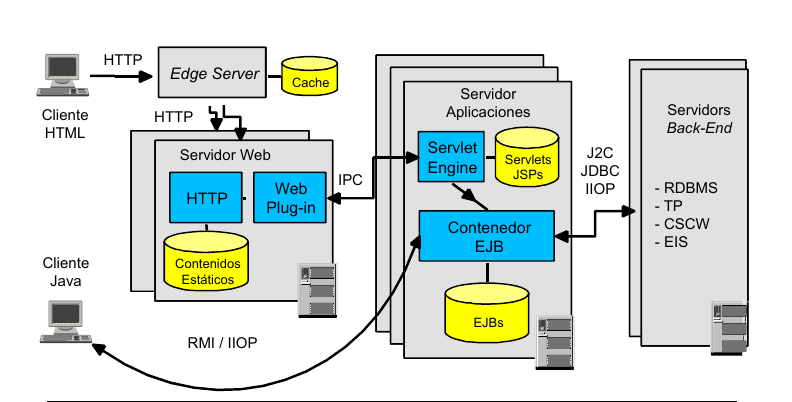
\includegraphics[width=\linewidth]{img/j2ee.png}
\end{center}

Se trata de un \textbf{cluster Activo-Activo}.

El balanceo de carga entre servidores Web lo realiza el Edge Server y el balanceo de carga entre Servlet Engines lo realiza el Web Plug In.

La alta disponibilidad en el acceso a los contenedores EJB y a los servicios de Back End es proporcionada por IIOP (corba) y por mecanismos de \textit{clustering} respectivamente.

La continuidad de la sesión entre distintas Servlet Engines se obtiene mediante el mantenimiento común de los datos de sesión. Este soporte común se puede conseguirse mediante una tabla de sesiones en una BD compartida, un gestor de réplica centralizado (Redundado para evitar SPOF) o un gestor de réplica distribuído.
\end{example}

\end{enumerate}

\section{Recuperación ante desastres}

Un desastre es cualquier circunstancia que puede producir un fallo en la operativa del negocio de una empresa. Pueden ser naturales, humanos, accidentes ...

Aunque tengan poca probabilidad, el impacto puede ser muy alto (por ejemplo, si se queman tus servidores de datos). Para garantizar la recuperación ante un desastre no basta con las técnicas de alta disponibilidad vistas hasta ahora sino que son necesarias nuevas técnicas que se presentan en esta sección.

Veamos algunas definiciones necesarias para entender los conceptos que analizaremos en este apartado:

\begin{defn}[Recovery\IS Point Objective (RPO)][Recovery\IS Point Objective]\index{RPO}
Instante de tiempo al que se es capaz de recuperar la información existente en el sistema tras un fallo. Si no es 0, habrá perdida de datos
\end{defn}

\begin{defn}[Recovery\IS Time Objective (RTO)][Recovery\IS Time Objective]\index{RTO}
Tiempo que se tarda en recuperar los sistemas tras producirse un fallo. Si no es 0, habrá interrupciones de servicio.
\end{defn}

Menores valores de RTO y RPO requieren mayor coste por lo que hay que analizar bien las necesidades del servicio.

Hay unas reglas básicas en el diseño de arquitecturas tolerantes a desastres:
\begin{enumerate}
\item Proteger datos y nodos de proceso mediante distribución geográfica.

Cuanto más alejados se encuentren, mayor seguridad, pero mayor
complejidad y coste.

\item Proporcionar a los CPDs redundancia en el suministro de energía.
Preferiblemente con acometidas independientes, a través de rutas alternativas de
distribución y proporcionadas por distintas entidades suministradoras.

\item Proporcionar a los CPDs redundancia en el acceso de telecomunicaciones. Con
las mismas consideraciones que en el caso anterior.

\item Generar copias consistentes de la información, garantizando la capacidad de
recuperar los datos desde ellas.
\begin{itemize}
\item \textbf{Copias off-line:} backups en cinta. Proporcionan un RPO elevado.

Puesto que hay que hacerlos de forma consistente, debe detenerse las aplicaciones mientras se realiza el backup o emplear técnicas de copia instantánea.

Además debe probarse que la información se restaura correctamente.

\item \textbf{Copias on-line:} réplicas directas de disco a disco. Proporcionan un RPO reducido.

Los mecanismos más habituales, ordenados de menor a mayor fiabilidad son:
\begin{enumerate}
\item Scripts de usuario. Automatizados por planificador.
\item Réplicas basadas en software en los sistemas de proceso, a distintos niveles:

\item Réplicas basadas en nivel de driver: mirroring remoto.
\item Réplicas basadas en el hardware de los servidores de disco: síncronas y
asíncronas, estudiadas previamente.
\end{enumerate}
\end{itemize}

\end{enumerate}

\subsection{Arquitecturas de CPDs orientadas a la recuperación ante desastres}
\textbf{Clusters a nivel de campus}
\begin{itemize}
\item Los elementos del cluster se distribuyen entre dos edificios próximos.
\item Extensión de LAN y SAN entre ambos edificios, normalmente con cableado propio.
\item Es posible la copia síncrona de información entre servidores de disco.
\item El funcionamiento lógico es como un cluster local: Proporciona alta disponibilidad.
\item Protege frente a desastres que ocurran en un único edificio.

\end{itemize}

\textbf{Clusters metropolitanos}
\begin{itemize}
\item Similar al anterior, pero con edificios en ubicaciones distantes que no excedan el rango en el que es posible realizar copia síncrona de la información.
\item Extensión de LAN y SAN con enlaces alquilados de alta velocidad (“fibra oscura”, WDM).
\item Protege frente a desastres locales.

\end{itemize}

\textbf{Clusters contienentales}
\begin{itemize}
\item Sin límite de distancia entre centros.
\item Requieren conexión a través de red WAN.
\item Protege frente a desastres en áreas extensas (región o estado), según la distancia entre centros.

\end{itemize}
\newpage
\textbf{Soluciones mixtas}
\begin{itemize}
\item Cluster local o metropolitano para garantizar alta disponibilidad, añadiendo un cluster continental para garantizar recuperación ante desastres.

\end{itemize}

\begin{center}
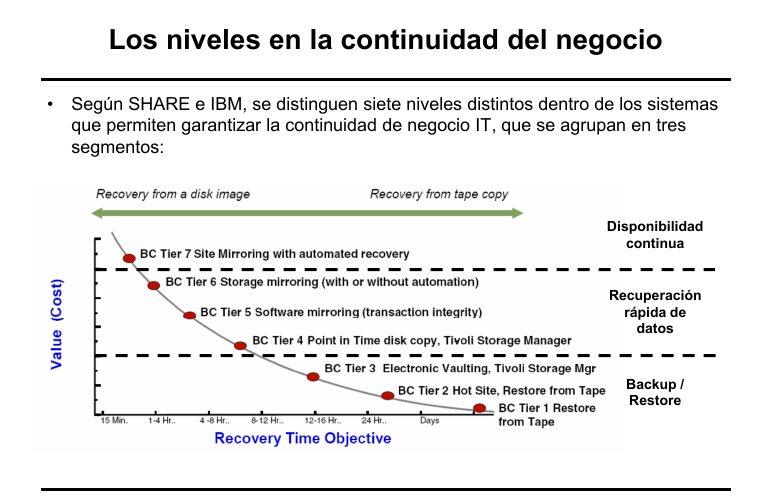
\includegraphics[width=\linewidth]{img/continuidad_negocio.png}
\end{center}

\end{document}
